% Options for packages loaded elsewhere
\PassOptionsToPackage{unicode}{hyperref}
\PassOptionsToPackage{hyphens}{url}
\PassOptionsToPackage{dvipsnames,svgnames,x11names}{xcolor}
%
\documentclass[
  letterpaper,
  DIV=11,
  numbers=noendperiod,
  oneside]{scrreprt}

\usepackage{amsmath,amssymb}
\usepackage{lmodern}
\usepackage{iftex}
\ifPDFTeX
  \usepackage[T1]{fontenc}
  \usepackage[utf8]{inputenc}
  \usepackage{textcomp} % provide euro and other symbols
\else % if luatex or xetex
  \usepackage{unicode-math}
  \defaultfontfeatures{Scale=MatchLowercase}
  \defaultfontfeatures[\rmfamily]{Ligatures=TeX,Scale=1}
\fi
% Use upquote if available, for straight quotes in verbatim environments
\IfFileExists{upquote.sty}{\usepackage{upquote}}{}
\IfFileExists{microtype.sty}{% use microtype if available
  \usepackage[]{microtype}
  \UseMicrotypeSet[protrusion]{basicmath} % disable protrusion for tt fonts
}{}
\makeatletter
\@ifundefined{KOMAClassName}{% if non-KOMA class
  \IfFileExists{parskip.sty}{%
    \usepackage{parskip}
  }{% else
    \setlength{\parindent}{0pt}
    \setlength{\parskip}{6pt plus 2pt minus 1pt}}
}{% if KOMA class
  \KOMAoptions{parskip=half}}
\makeatother
\usepackage{xcolor}
\usepackage[left=1in,marginparwidth=2.0666666666667in,textwidth=4.1333333333333in,marginparsep=0.3in]{geometry}
\setlength{\emergencystretch}{3em} % prevent overfull lines
\setcounter{secnumdepth}{5}
% Make \paragraph and \subparagraph free-standing
\ifx\paragraph\undefined\else
  \let\oldparagraph\paragraph
  \renewcommand{\paragraph}[1]{\oldparagraph{#1}\mbox{}}
\fi
\ifx\subparagraph\undefined\else
  \let\oldsubparagraph\subparagraph
  \renewcommand{\subparagraph}[1]{\oldsubparagraph{#1}\mbox{}}
\fi

\usepackage{color}
\usepackage{fancyvrb}
\newcommand{\VerbBar}{|}
\newcommand{\VERB}{\Verb[commandchars=\\\{\}]}
\DefineVerbatimEnvironment{Highlighting}{Verbatim}{commandchars=\\\{\}}
% Add ',fontsize=\small' for more characters per line
\usepackage{framed}
\definecolor{shadecolor}{RGB}{241,243,245}
\newenvironment{Shaded}{\begin{snugshade}}{\end{snugshade}}
\newcommand{\AlertTok}[1]{\textcolor[rgb]{0.68,0.00,0.00}{#1}}
\newcommand{\AnnotationTok}[1]{\textcolor[rgb]{0.37,0.37,0.37}{#1}}
\newcommand{\AttributeTok}[1]{\textcolor[rgb]{0.40,0.45,0.13}{#1}}
\newcommand{\BaseNTok}[1]{\textcolor[rgb]{0.68,0.00,0.00}{#1}}
\newcommand{\BuiltInTok}[1]{\textcolor[rgb]{0.00,0.23,0.31}{#1}}
\newcommand{\CharTok}[1]{\textcolor[rgb]{0.13,0.47,0.30}{#1}}
\newcommand{\CommentTok}[1]{\textcolor[rgb]{0.37,0.37,0.37}{#1}}
\newcommand{\CommentVarTok}[1]{\textcolor[rgb]{0.37,0.37,0.37}{\textit{#1}}}
\newcommand{\ConstantTok}[1]{\textcolor[rgb]{0.56,0.35,0.01}{#1}}
\newcommand{\ControlFlowTok}[1]{\textcolor[rgb]{0.00,0.23,0.31}{#1}}
\newcommand{\DataTypeTok}[1]{\textcolor[rgb]{0.68,0.00,0.00}{#1}}
\newcommand{\DecValTok}[1]{\textcolor[rgb]{0.68,0.00,0.00}{#1}}
\newcommand{\DocumentationTok}[1]{\textcolor[rgb]{0.37,0.37,0.37}{\textit{#1}}}
\newcommand{\ErrorTok}[1]{\textcolor[rgb]{0.68,0.00,0.00}{#1}}
\newcommand{\ExtensionTok}[1]{\textcolor[rgb]{0.00,0.23,0.31}{#1}}
\newcommand{\FloatTok}[1]{\textcolor[rgb]{0.68,0.00,0.00}{#1}}
\newcommand{\FunctionTok}[1]{\textcolor[rgb]{0.28,0.35,0.67}{#1}}
\newcommand{\ImportTok}[1]{\textcolor[rgb]{0.00,0.46,0.62}{#1}}
\newcommand{\InformationTok}[1]{\textcolor[rgb]{0.37,0.37,0.37}{#1}}
\newcommand{\KeywordTok}[1]{\textcolor[rgb]{0.00,0.23,0.31}{#1}}
\newcommand{\NormalTok}[1]{\textcolor[rgb]{0.00,0.23,0.31}{#1}}
\newcommand{\OperatorTok}[1]{\textcolor[rgb]{0.37,0.37,0.37}{#1}}
\newcommand{\OtherTok}[1]{\textcolor[rgb]{0.00,0.23,0.31}{#1}}
\newcommand{\PreprocessorTok}[1]{\textcolor[rgb]{0.68,0.00,0.00}{#1}}
\newcommand{\RegionMarkerTok}[1]{\textcolor[rgb]{0.00,0.23,0.31}{#1}}
\newcommand{\SpecialCharTok}[1]{\textcolor[rgb]{0.37,0.37,0.37}{#1}}
\newcommand{\SpecialStringTok}[1]{\textcolor[rgb]{0.13,0.47,0.30}{#1}}
\newcommand{\StringTok}[1]{\textcolor[rgb]{0.13,0.47,0.30}{#1}}
\newcommand{\VariableTok}[1]{\textcolor[rgb]{0.07,0.07,0.07}{#1}}
\newcommand{\VerbatimStringTok}[1]{\textcolor[rgb]{0.13,0.47,0.30}{#1}}
\newcommand{\WarningTok}[1]{\textcolor[rgb]{0.37,0.37,0.37}{\textit{#1}}}

\providecommand{\tightlist}{%
  \setlength{\itemsep}{0pt}\setlength{\parskip}{0pt}}\usepackage{longtable,booktabs,array}
\usepackage{calc} % for calculating minipage widths
% Correct order of tables after \paragraph or \subparagraph
\usepackage{etoolbox}
\makeatletter
\patchcmd\longtable{\par}{\if@noskipsec\mbox{}\fi\par}{}{}
\makeatother
% Allow footnotes in longtable head/foot
\IfFileExists{footnotehyper.sty}{\usepackage{footnotehyper}}{\usepackage{footnote}}
\makesavenoteenv{longtable}
\usepackage{graphicx}
\makeatletter
\def\maxwidth{\ifdim\Gin@nat@width>\linewidth\linewidth\else\Gin@nat@width\fi}
\def\maxheight{\ifdim\Gin@nat@height>\textheight\textheight\else\Gin@nat@height\fi}
\makeatother
% Scale images if necessary, so that they will not overflow the page
% margins by default, and it is still possible to overwrite the defaults
% using explicit options in \includegraphics[width, height, ...]{}
\setkeys{Gin}{width=\maxwidth,height=\maxheight,keepaspectratio}
% Set default figure placement to htbp
\makeatletter
\def\fps@figure{htbp}
\makeatother
\newlength{\cslhangindent}
\setlength{\cslhangindent}{1.5em}
\newlength{\csllabelwidth}
\setlength{\csllabelwidth}{3em}
\newlength{\cslentryspacingunit} % times entry-spacing
\setlength{\cslentryspacingunit}{\parskip}
\newenvironment{CSLReferences}[2] % #1 hanging-ident, #2 entry spacing
 {% don't indent paragraphs
  \setlength{\parindent}{0pt}
  % turn on hanging indent if param 1 is 1
  \ifodd #1
  \let\oldpar\par
  \def\par{\hangindent=\cslhangindent\oldpar}
  \fi
  % set entry spacing
  \setlength{\parskip}{#2\cslentryspacingunit}
 }%
 {}
\usepackage{calc}
\newcommand{\CSLBlock}[1]{#1\hfill\break}
\newcommand{\CSLLeftMargin}[1]{\parbox[t]{\csllabelwidth}{#1}}
\newcommand{\CSLRightInline}[1]{\parbox[t]{\linewidth - \csllabelwidth}{#1}\break}
\newcommand{\CSLIndent}[1]{\hspace{\cslhangindent}#1}

\KOMAoption{captions}{tableheading}
\makeatletter
\makeatother
\makeatletter
\@ifpackageloaded{bookmark}{}{\usepackage{bookmark}}
\makeatother
\makeatletter
\@ifpackageloaded{caption}{}{\usepackage{caption}}
\AtBeginDocument{%
\ifdefined\contentsname
  \renewcommand*\contentsname{Table of contents}
\else
  \newcommand\contentsname{Table of contents}
\fi
\ifdefined\listfigurename
  \renewcommand*\listfigurename{List of Figures}
\else
  \newcommand\listfigurename{List of Figures}
\fi
\ifdefined\listtablename
  \renewcommand*\listtablename{List of Tables}
\else
  \newcommand\listtablename{List of Tables}
\fi
\ifdefined\figurename
  \renewcommand*\figurename{Figure}
\else
  \newcommand\figurename{Figure}
\fi
\ifdefined\tablename
  \renewcommand*\tablename{Table}
\else
  \newcommand\tablename{Table}
\fi
}
\@ifpackageloaded{float}{}{\usepackage{float}}
\floatstyle{ruled}
\@ifundefined{c@chapter}{\newfloat{codelisting}{h}{lop}}{\newfloat{codelisting}{h}{lop}[chapter]}
\floatname{codelisting}{Listing}
\newcommand*\listoflistings{\listof{codelisting}{List of Listings}}
\makeatother
\makeatletter
\@ifpackageloaded{caption}{}{\usepackage{caption}}
\@ifpackageloaded{subcaption}{}{\usepackage{subcaption}}
\makeatother
\makeatletter
\@ifpackageloaded{tcolorbox}{}{\usepackage[many]{tcolorbox}}
\makeatother
\makeatletter
\@ifundefined{shadecolor}{\definecolor{shadecolor}{rgb}{.97, .97, .97}}
\makeatother
\makeatletter
\@ifpackageloaded{sidenotes}{}{\usepackage{sidenotes}}
\@ifpackageloaded{marginnote}{}{\usepackage{marginnote}}
\makeatother
\makeatletter
\makeatother
\ifLuaTeX
  \usepackage{selnolig}  % disable illegal ligatures
\fi
\IfFileExists{bookmark.sty}{\usepackage{bookmark}}{\usepackage{hyperref}}
\IfFileExists{xurl.sty}{\usepackage{xurl}}{} % add URL line breaks if available
\urlstyle{same} % disable monospaced font for URLs
\hypersetup{
  pdftitle={Time Series Analysis},
  pdfauthor={Yair Mau},
  colorlinks=true,
  linkcolor={blue},
  filecolor={Maroon},
  citecolor={Blue},
  urlcolor={Blue},
  pdfcreator={LaTeX via pandoc}}

\title{Time Series Analysis}
\author{Yair Mau}
\date{}

\begin{document}
\maketitle
\ifdefined\Shaded\renewenvironment{Shaded}{\begin{tcolorbox}[interior hidden, borderline west={3pt}{0pt}{shadecolor}, boxrule=0pt, enhanced, sharp corners, breakable, frame hidden]}{\end{tcolorbox}}\fi

\renewcommand*\contentsname{Table of contents}
{
\hypersetup{linkcolor=}
\setcounter{tocdepth}{2}
\tableofcontents
}
\bookmarksetup{startatroot}

\hypertarget{about}{%
\chapter*{About}\label{about}}
\addcontentsline{toc}{chapter}{About}

\markboth{About}{About}

Welcome to Time Series Analysis for Environmental Sciences (71606) at
the Hebrew University of Jerusalem. This is Yair Mau, your host for
today. I am a senior lecturer at the Institute of Environmental
Sciences, at the Faculty of Agriculture, Food and Environment, in
Rehovot, Israel.

This website contains (almost) all the material you'll need for the
course. If you find any mistakes, or have any comments, please email me.

\hypertarget{disclaimer}{%
\section*{Disclaimer}\label{disclaimer}}
\addcontentsline{toc}{section}{Disclaimer}

\markright{Disclaimer}

The material here is not comprehensive and \texttt{does\ not} constitute
a stand alone course in Time Series Analysis. This is only the support
material for the actual presential course I give.

\hypertarget{what-who-when-and-where}{%
\section*{What, who, when and where?}\label{what-who-when-and-where}}
\addcontentsline{toc}{section}{What, who, when and where?}

\markright{What, who, when and where?}

Course number 71606, 3 academic points\\
Yair Mau (lecturer), Erez Feuer (TA)\\
Tuesdays, from 14:15 to 17:00\\
Computer \href{https://goo.gl/maps/21CScuxTqJ28Umjw5}{classroom \#16}\\
Office hours: upon request

\hypertarget{syllabus}{%
\section*{Syllabus}\label{syllabus}}
\addcontentsline{toc}{section}{Syllabus}

\markright{Syllabus}

\hypertarget{course-description}{%
\subsection*{Course description}\label{course-description}}
\addcontentsline{toc}{subsection}{Course description}

Data analysis of time series, with practical examples from environmental
sciences.

\hypertarget{course-aims}{%
\subsection*{Course aims}\label{course-aims}}
\addcontentsline{toc}{subsection}{Course aims}

This course aims at giving the students a broad overview of the main
steps involved in the analysis of time series: data management, data
wrangling, visualization, analysis, and forecast. The course will
provide a hands-on approach, where students will actively engage with
real-life datasets from the field of environmental science.

\hypertarget{learning-outcomes}{%
\subsection*{Learning outcomes}\label{learning-outcomes}}
\addcontentsline{toc}{subsection}{Learning outcomes}

On successful completion of this module,students should be able to:

\begin{itemize}
\tightlist
\item
  Explore a time-series dataset, while formulating interesting
  questions.
\item
  Choose the appropriate tools to attack the problem and answer the
  questions.
\item
  Communicate their findings and the methods they used to achieve them,
  using graphs, statistics, text, and a well-documented code.
\end{itemize}

\hypertarget{course-content}{%
\subsection*{Course content}\label{course-content}}
\addcontentsline{toc}{subsection}{Course content}

\begin{itemize}
\tightlist
\item
  \textbf{Data wrangling:} organization, cleaning, merging, filling
  gaps, excluding outliers, smoothing, resampling.
\item
  \textbf{Visualization:} best practices for graph making using leading
  python libraries.
\item
  \textbf{Analysis:} stationarity, seasonality, (auto)correlations,
  lags, derivatives, spectral analysis.
\item
  \textbf{Forecast:} ARIMA
\item
  \textbf{Data management:} how to plan ahead and best organize large
  quantities of data. If there is enough time, we will build a simple
  time-series database.
\end{itemize}

\hypertarget{books-and-other-sources}{%
\subsection*{Books and other sources}\label{books-and-other-sources}}
\addcontentsline{toc}{subsection}{Books and other sources}

\href{references.html}{Click here.}

\hypertarget{course-evaluation}{%
\subsection*{Course evaluation}\label{course-evaluation}}
\addcontentsline{toc}{subsection}{Course evaluation}

There will be 2 projects during the semester (each worth 25\% of the
final grade), and one final project (50\%).

\hypertarget{weekly-program}{%
\section*{Weekly program}\label{weekly-program}}
\addcontentsline{toc}{section}{Weekly program}

\markright{Weekly program}

\hypertarget{week-1}{%
\subsubsection*{Week 1}\label{week-1}}
\addcontentsline{toc}{subsubsection}{Week 1}

\begin{itemize}
\tightlist
\item
  \textbf{Lecture:} Course overview, setting of expectations.
  Introduction, basic concepts, continuous vs discrete time series,
  sampling, aliasing
\item
  \textbf{Exercise:} Loading csv file into python, basic time series
  manipulation with pandas and plotting
\end{itemize}

\hypertarget{week-2}{%
\subsubsection*{Week 2}\label{week-2}}
\addcontentsline{toc}{subsubsection}{Week 2}

\begin{itemize}
\tightlist
\item
  \textbf{Lecture:} Filling gaps, removing outliers
\item
  \textbf{Exercise:} Practice the same topics learned during the
  lecture. Data: air temperature and relative humidity
\end{itemize}

\hypertarget{week-3}{%
\subsubsection*{Week 3}\label{week-3}}
\addcontentsline{toc}{subsubsection}{Week 3}

\begin{itemize}
\tightlist
\item
  \textbf{Lecture:} Interpolation, resampling, binning statistics
\item
  \textbf{Exercise:} Practice the same topics learned during the
  lecture. Data: air temperature and relative humidity, precipitation
\end{itemize}

\hypertarget{week-4}{%
\subsubsection*{Week 4}\label{week-4}}
\addcontentsline{toc}{subsubsection}{Week 4}

\begin{itemize}
\tightlist
\item
  \textbf{Lecture:} Time series plotting: best practices. Dos and don'ts
  and maybes
\item
  \textbf{Exercise:} Practice with Seaborn, Plotly, Pandas, Matplotlib
\end{itemize}

\textbf{Project 1}\\
Basic data wrangling, using real data (temperature, relative humidity,
precipitation) downloaded from USGS. 25\% of the final grade

\hypertarget{week-5}{%
\subsubsection*{Week 5}\label{week-5}}
\addcontentsline{toc}{subsubsection}{Week 5}

\begin{itemize}
\tightlist
\item
  \textbf{Lecture:} Smoothing, running averages, convolution
\item
  \textbf{Exercise:} Practice the same topics learned during the
  lecture. Data: sap flow, evapotranspiration
\end{itemize}

\hypertarget{week-6}{%
\subsubsection*{Week 6}\label{week-6}}
\addcontentsline{toc}{subsubsection}{Week 6}

\begin{itemize}
\tightlist
\item
  \textbf{Lecture:} Strong and weak stationarity, stochastic processes,
  auto-correlation
\item
  \textbf{Exercise:} Practice the same topics learned during the
  lecture. Data: temperature and wind speed
\end{itemize}

\hypertarget{week-7}{%
\subsubsection*{Week 7}\label{week-7}}
\addcontentsline{toc}{subsubsection}{Week 7}

\begin{itemize}
\tightlist
\item
  \textbf{Lecture:} Correlation between signals. Pearson correlation,
  time-lagged cross-correlations, dynamic time warping
\item
  \textbf{Exercise:} Practice the same topics learned during the
  lecture. Data: temperature, solar radiation, relative humidity, soil
  moisture, evapotranspiration
\end{itemize}

\hypertarget{week-8}{%
\subsubsection*{Week 8}\label{week-8}}
\addcontentsline{toc}{subsubsection}{Week 8}

Same as lecture 7 above

\hypertarget{week-9}{%
\subsubsection*{Week 9}\label{week-9}}
\addcontentsline{toc}{subsubsection}{Week 9}

\begin{itemize}
\tightlist
\item
  \textbf{Lecture:} Download data from repositories, using API, merging,
  documentation
\item
  \textbf{Exercise:} Download data from USGS, NOAA, Fluxnet, Israel
  Meteorological Service
\end{itemize}

\textbf{Project 2}\\
Students will study a Fluxnet site of their choosing. How do gas fluxes
(CO2, H2O) depend on environmental conditions? 25\% of the final grade

\hypertarget{week-10}{%
\subsubsection*{Week 10}\label{week-10}}
\addcontentsline{toc}{subsubsection}{Week 10}

\begin{itemize}
\tightlist
\item
  \textbf{Lecture:} Fourier decomposition, filtering, Nyquist--Shannon
  sampling theorem
\item
  \textbf{Exercise:} Practice the same topics learned during the
  lecture. Data: dendrometer data
\end{itemize}

\hypertarget{week-11}{%
\subsubsection*{Week 11}\label{week-11}}
\addcontentsline{toc}{subsubsection}{Week 11}

\begin{itemize}
\tightlist
\item
  \textbf{Lecture:} Seasonality, seasonal decomposition (trend,
  seasonal, residue), Hilbert transform
\item
  \textbf{Exercise:} Practice the same topics learned during the
  lecture. Data: monthly atmospheric CO2 concentration, hourly air
  temperature
\end{itemize}

\hypertarget{week-12}{%
\subsubsection*{Week 12}\label{week-12}}
\addcontentsline{toc}{subsubsection}{Week 12}

\begin{itemize}
\tightlist
\item
  \textbf{Lecture:} Derivatives, differencing
\item
  \textbf{Exercise:} Practice the same topics learned during the
  lecture. Data: dendrometer data
\end{itemize}

\hypertarget{week-13}{%
\subsubsection*{Week 13}\label{week-13}}
\addcontentsline{toc}{subsubsection}{Week 13}

\begin{itemize}
\tightlist
\item
  \textbf{Lecture:} Forecasting. ARIMA
\item
  \textbf{Exercise:} Practice the same topics learned during the
  lecture. Data: vegetation variables (sap flow, ET, DBH, etc)
\end{itemize}

\textbf{Final Project}\\
In consultation with the lecturer, students will ask a specific
scientific question about a site of their choosing (from NOAA, USGS,
Fluxnet), and answer it using the tools learned during the semester. The
report will be written in Jupyter Notebook, combining in one document
all the calculations, documentation, figures, analysis, and discussion.
50\% of the final grade.

\part{Basic data manipulation and plotting}

\hypertarget{pandas}{%
\chapter{Pandas}\label{pandas}}

\hypertarget{pyplot}{%
\chapter{Pyplot}\label{pyplot}}

\hypertarget{first-steps-basic-time-series-analysis}{%
\chapter{First Steps --- basic time series
analysis}\label{first-steps-basic-time-series-analysis}}

Import packages. If you don't have a certain package, e.g.~`newpackage',
just type\\
\texttt{pip\ install\ newpackage}

\begin{Shaded}
\begin{Highlighting}[]
\ImportTok{import}\NormalTok{ urllib}
\ImportTok{import}\NormalTok{ matplotlib.pyplot }\ImportTok{as}\NormalTok{ plt}
\ImportTok{import}\NormalTok{ numpy }\ImportTok{as}\NormalTok{ np}
\ImportTok{import}\NormalTok{ pandas }\ImportTok{as}\NormalTok{ pd}
\ImportTok{import}\NormalTok{ os.path}
\ImportTok{import}\NormalTok{ matplotlib.dates }\ImportTok{as}\NormalTok{ mdates}
\ImportTok{import}\NormalTok{ datetime }\ImportTok{as}\NormalTok{ dt}
\ImportTok{import}\NormalTok{ matplotlib }\ImportTok{as}\NormalTok{ mpl}
\ImportTok{from}\NormalTok{ pandas.tseries.frequencies }\ImportTok{import}\NormalTok{ to\_offset}
\ImportTok{from}\NormalTok{ scipy.signal }\ImportTok{import}\NormalTok{ savgol\_filter}
\end{Highlighting}
\end{Shaded}

This is how you download data from Thingspeak

\begin{Shaded}
\begin{Highlighting}[]
\NormalTok{filename1 }\OperatorTok{=} \StringTok{"test\_elad.csv"}
\CommentTok{\# if file is not there, go fetch it from thingspeak}
\ControlFlowTok{if} \KeywordTok{not}\NormalTok{ os.path.isfile(filename1):}
    \CommentTok{\# define what to download}
\NormalTok{    channels }\OperatorTok{=} \StringTok{"1690490"}
\NormalTok{    fields }\OperatorTok{=} \StringTok{"1,2,3,4,6,7"}
\NormalTok{    minutes }\OperatorTok{=} \StringTok{"30"}

    \CommentTok{\# https://www.mathworks.com/help/thingspeak/readdata.html}
    \CommentTok{\# format YYYY{-}MM{-}DD\%20HH:NN:SS}
\NormalTok{    start }\OperatorTok{=} \StringTok{"2022{-}05{-}01\%2000:00:00"}
\NormalTok{    end }\OperatorTok{=} \StringTok{"2022{-}05{-}08\%2000:00:00"}

    \CommentTok{\# download using Thingspeak\textquotesingle{}s API}
    \CommentTok{\# url = f"https://api.thingspeak.com/channels/\{channels\}/fields/\{fields\}.csv?minutes=\{minutes\}"}
\NormalTok{    url }\OperatorTok{=} \SpecialStringTok{f"https://api.thingspeak.com/channels/}\SpecialCharTok{\{}\NormalTok{channels}\SpecialCharTok{\}}\SpecialStringTok{/fields/}\SpecialCharTok{\{}\NormalTok{fields}\SpecialCharTok{\}}\SpecialStringTok{.csv?start=}\SpecialCharTok{\{}\NormalTok{start}\SpecialCharTok{\}}\SpecialStringTok{\&end=}\SpecialCharTok{\{}\NormalTok{end}\SpecialCharTok{\}}\SpecialStringTok{"}
\NormalTok{    data }\OperatorTok{=}\NormalTok{ urllib.request.urlopen(url)}
\NormalTok{    d }\OperatorTok{=}\NormalTok{ data.read()}

    \CommentTok{\# save data to csv}
    \BuiltInTok{file} \OperatorTok{=} \BuiltInTok{open}\NormalTok{(filename1, }\StringTok{"w"}\NormalTok{)}
    \BuiltInTok{file}\NormalTok{.write(d.decode(}\StringTok{\textquotesingle{}UTF{-}8\textquotesingle{}}\NormalTok{))}
    \BuiltInTok{file}\NormalTok{.close()}
\end{Highlighting}
\end{Shaded}

You can load the data using Pandas. Here we create a ``dataframe'',
which is a fancy name for a table.

\begin{Shaded}
\begin{Highlighting}[]
\CommentTok{\# load data}
\NormalTok{df }\OperatorTok{=}\NormalTok{ pd.read\_csv(filename1)}
\CommentTok{\# rename columns}
\NormalTok{df }\OperatorTok{=}\NormalTok{ df.rename(columns}\OperatorTok{=}\NormalTok{\{}\StringTok{"created\_at"}\NormalTok{: }\StringTok{"timestamp"}\NormalTok{,}
                        \StringTok{"field1"}\NormalTok{: }\StringTok{"T1"}\NormalTok{,}
                        \StringTok{"field2"}\NormalTok{: }\StringTok{"RH"}\NormalTok{,}
                        \StringTok{"field3"}\NormalTok{: }\StringTok{"T2"}\NormalTok{,}
                        \StringTok{"field4"}\NormalTok{: }\StringTok{"motion\_sensor"}\NormalTok{,}
                        \StringTok{"field6"}\NormalTok{: }\StringTok{"VWC"}\NormalTok{,}
                        \StringTok{"field7"}\NormalTok{: }\StringTok{"VPD"}\NormalTok{,\})}
\CommentTok{\# set timestamp as index}
\NormalTok{df[}\StringTok{\textquotesingle{}timestamp\textquotesingle{}}\NormalTok{] }\OperatorTok{=}\NormalTok{ pd.to\_datetime(df[}\StringTok{\textquotesingle{}timestamp\textquotesingle{}}\NormalTok{])}
\NormalTok{df }\OperatorTok{=}\NormalTok{ df.set\_index(}\StringTok{\textquotesingle{}timestamp\textquotesingle{}}\NormalTok{)}
\end{Highlighting}
\end{Shaded}

\hypertarget{first-graph}{%
\subsection{First graph}\label{first-graph}}

\begin{Shaded}
\begin{Highlighting}[]
\CommentTok{\# \%matplotlib widget}

\NormalTok{fig, ax }\OperatorTok{=}\NormalTok{ plt.subplots(}\DecValTok{1}\NormalTok{, figsize}\OperatorTok{=}\NormalTok{(}\DecValTok{8}\NormalTok{,}\DecValTok{6}\NormalTok{))}

\NormalTok{ax.plot(df[}\StringTok{\textquotesingle{}VPD\textquotesingle{}}\NormalTok{])}
\CommentTok{\# add labels and title}
\NormalTok{ax.}\BuiltInTok{set}\NormalTok{(xlabel }\OperatorTok{=} \StringTok{"time"}\NormalTok{,}
\NormalTok{       ylabel }\OperatorTok{=} \StringTok{"VPD (kPa)"}\NormalTok{,}
\NormalTok{       title }\OperatorTok{=} \StringTok{"my first graph"}\NormalTok{)}
\CommentTok{\# makes slanted dates}
\NormalTok{plt.gcf().autofmt\_xdate()  }
\end{Highlighting}
\end{Shaded}

\begin{figure}[H]

{\centering \includegraphics{introduction/first-steps_files/figure-pdf/cell-5-output-1.png}

}

\end{figure}

\hypertarget{two-columns-in-the-same-graph}{%
\subsection{Two columns in the same
graph}\label{two-columns-in-the-same-graph}}

\begin{Shaded}
\begin{Highlighting}[]
\CommentTok{\# \%matplotlib widget}

\NormalTok{fig, ax }\OperatorTok{=}\NormalTok{ plt.subplots(}\DecValTok{1}\NormalTok{, figsize}\OperatorTok{=}\NormalTok{(}\DecValTok{8}\NormalTok{,}\DecValTok{6}\NormalTok{))}

\NormalTok{ax.plot(df[}\StringTok{\textquotesingle{}T1\textquotesingle{}}\NormalTok{], color}\OperatorTok{=}\StringTok{"tab:blue"}\NormalTok{, label}\OperatorTok{=}\StringTok{"SHT Temperature"}\NormalTok{)}
\NormalTok{ax.plot(df[}\StringTok{\textquotesingle{}T2\textquotesingle{}}\NormalTok{], color}\OperatorTok{=}\StringTok{"tab:orange"}\NormalTok{, label}\OperatorTok{=}\StringTok{"DS18B20 Temperature"}\NormalTok{)}
\CommentTok{\# add labels and title}
\NormalTok{ax.}\BuiltInTok{set}\NormalTok{(xlabel }\OperatorTok{=} \StringTok{"Time"}\NormalTok{,}
\NormalTok{       ylabel }\OperatorTok{=} \StringTok{"Temperature (deg C)"}\NormalTok{,}
\NormalTok{       title }\OperatorTok{=} \StringTok{"two sensors"}\NormalTok{,}
\NormalTok{       ylim}\OperatorTok{=}\NormalTok{[}\DecValTok{20}\NormalTok{,}\DecValTok{35}\NormalTok{],}
\NormalTok{       )}
\CommentTok{\# makes slanted dates}
\NormalTok{plt.gcf().autofmt\_xdate()}
\NormalTok{ax.legend(loc}\OperatorTok{=}\StringTok{"upper right"}\NormalTok{)}
\end{Highlighting}
\end{Shaded}

\begin{verbatim}
<matplotlib.legend.Legend at 0x7fe6c9730610>
\end{verbatim}

\begin{figure}[H]

{\centering 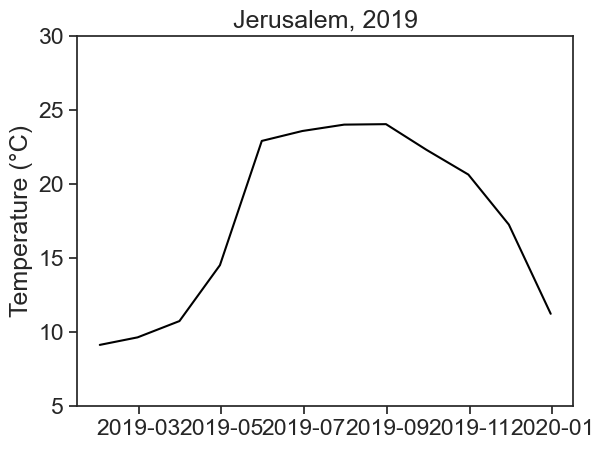
\includegraphics{introduction/first-steps_files/figure-pdf/cell-6-output-2.png}

}

\end{figure}

\hypertarget{calculate-stuff}{%
\subsection{Calculate stuff}\label{calculate-stuff}}

You can calculate new things and save them as new columns of your
dataframe.

\begin{Shaded}
\begin{Highlighting}[]
\KeywordTok{def}\NormalTok{ calculate\_es(T):}
\NormalTok{    es }\OperatorTok{=}\NormalTok{ np.exp((}\FloatTok{16.78} \OperatorTok{*}\NormalTok{ T }\OperatorTok{{-}} \FloatTok{116.9}\NormalTok{) }\OperatorTok{/}\NormalTok{ (T }\OperatorTok{+} \FloatTok{237.3}\NormalTok{))}
    \ControlFlowTok{return}\NormalTok{ es}

\KeywordTok{def}\NormalTok{ calculate\_ed(es, rh):}
    \ControlFlowTok{return}\NormalTok{ es }\OperatorTok{*}\NormalTok{ rh }\OperatorTok{/} \FloatTok{100.0}

\NormalTok{es }\OperatorTok{=}\NormalTok{ calculate\_es(df[}\StringTok{\textquotesingle{}T1\textquotesingle{}}\NormalTok{])}
\NormalTok{ed }\OperatorTok{=}\NormalTok{ calculate\_ed(es, df[}\StringTok{\textquotesingle{}RH\textquotesingle{}}\NormalTok{])}
\NormalTok{df[}\StringTok{\textquotesingle{}VPD2\textquotesingle{}}\NormalTok{] }\OperatorTok{=}\NormalTok{ es }\OperatorTok{{-}}\NormalTok{ ed}
\end{Highlighting}
\end{Shaded}

See if what you calculated makes sense.

\begin{Shaded}
\begin{Highlighting}[]
\CommentTok{\# \%matplotlib widget}

\NormalTok{fig, ax }\OperatorTok{=}\NormalTok{ plt.subplots(}\DecValTok{1}\NormalTok{, figsize}\OperatorTok{=}\NormalTok{(}\DecValTok{8}\NormalTok{,}\DecValTok{6}\NormalTok{))}

\NormalTok{ax.plot(df[}\StringTok{\textquotesingle{}VPD\textquotesingle{}}\NormalTok{], color}\OperatorTok{=}\StringTok{"tab:red"}\NormalTok{, label}\OperatorTok{=}\StringTok{"VPD from ESP32"}\NormalTok{)}
\NormalTok{ax.plot(df[}\StringTok{\textquotesingle{}VPD2\textquotesingle{}}\NormalTok{][::}\DecValTok{100}\NormalTok{], }\StringTok{"o"}\NormalTok{, color}\OperatorTok{=}\StringTok{"black"}\NormalTok{, label}\OperatorTok{=}\StringTok{"VPD from python"}\NormalTok{)}
\CommentTok{\# add labels and title}
\NormalTok{ax.}\BuiltInTok{set}\NormalTok{(xlabel }\OperatorTok{=} \StringTok{"Time"}\NormalTok{,}
\NormalTok{       ylabel }\OperatorTok{=} \StringTok{"VPD (kPa)"}\NormalTok{,}
\NormalTok{       title }\OperatorTok{=} \StringTok{"VPD calculated twice"}\NormalTok{,}
\NormalTok{       ylim}\OperatorTok{=}\NormalTok{[}\DecValTok{0}\NormalTok{,}\DecValTok{5}\NormalTok{],}
\NormalTok{       )}
\CommentTok{\# makes slanted dates}
\NormalTok{plt.gcf().autofmt\_xdate()}
\NormalTok{ax.legend(loc}\OperatorTok{=}\StringTok{"upper right"}\NormalTok{)}
\end{Highlighting}
\end{Shaded}

\begin{verbatim}
<matplotlib.legend.Legend at 0x7fe6989ca700>
\end{verbatim}

\begin{figure}[H]

{\centering 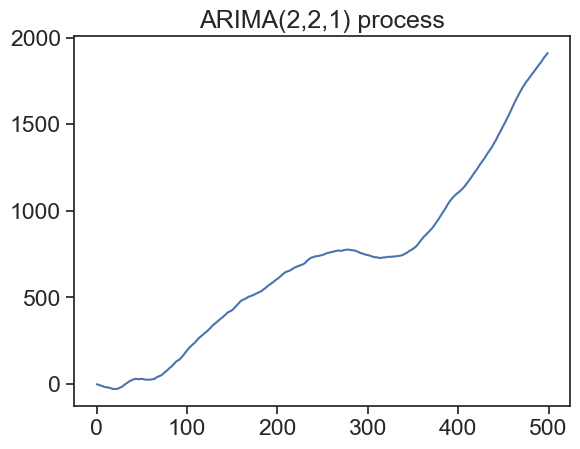
\includegraphics{introduction/first-steps_files/figure-pdf/cell-8-output-2.png}

}

\end{figure}

\hypertarget{two-y-axes}{%
\subsection{Two y axes}\label{two-y-axes}}

\begin{Shaded}
\begin{Highlighting}[]
\CommentTok{\# \%matplotlib widget}

\NormalTok{fig, ax }\OperatorTok{=}\NormalTok{ plt.subplots(}\DecValTok{1}\NormalTok{, figsize}\OperatorTok{=}\NormalTok{(}\DecValTok{8}\NormalTok{,}\DecValTok{6}\NormalTok{))}

\NormalTok{ax.plot(df[}\StringTok{\textquotesingle{}VPD\textquotesingle{}}\NormalTok{], color}\OperatorTok{=}\StringTok{"tab:red"}\NormalTok{, label}\OperatorTok{=}\StringTok{"VPD"}\NormalTok{)}
\NormalTok{plt.gcf().autofmt\_xdate()}
\NormalTok{ax2 }\OperatorTok{=}\NormalTok{ ax.twinx()}
\NormalTok{ax2.plot(df[}\StringTok{\textquotesingle{}T1\textquotesingle{}}\NormalTok{], color}\OperatorTok{=}\StringTok{"tab:cyan"}\NormalTok{, label}\OperatorTok{=}\StringTok{"Temperature"}\NormalTok{)}
\NormalTok{ax.}\BuiltInTok{set}\NormalTok{(xlabel }\OperatorTok{=} \StringTok{"Time"}\NormalTok{,}
\NormalTok{       title }\OperatorTok{=} \StringTok{"two y axes"}\NormalTok{,}
\NormalTok{       ylim}\OperatorTok{=}\NormalTok{[}\DecValTok{0}\NormalTok{,}\DecValTok{5}\NormalTok{],}
\NormalTok{       )}
\NormalTok{ax.set\_ylabel(}\StringTok{\textquotesingle{}VPD (kPa)\textquotesingle{}}\NormalTok{, color}\OperatorTok{=}\StringTok{\textquotesingle{}tab:red\textquotesingle{}}\NormalTok{)}
\NormalTok{ax.spines[}\StringTok{\textquotesingle{}left\textquotesingle{}}\NormalTok{].set\_color(}\StringTok{\textquotesingle{}red\textquotesingle{}}\NormalTok{)}

\NormalTok{ax2.set\_ylabel(}\StringTok{\textquotesingle{}Temperature (deg C)\textquotesingle{}}\NormalTok{, color}\OperatorTok{=}\StringTok{\textquotesingle{}tab:cyan\textquotesingle{}}\NormalTok{)}
\end{Highlighting}
\end{Shaded}

\begin{verbatim}
Text(0, 0.5, 'Temperature (deg C)')
\end{verbatim}

\begin{figure}[H]

{\centering 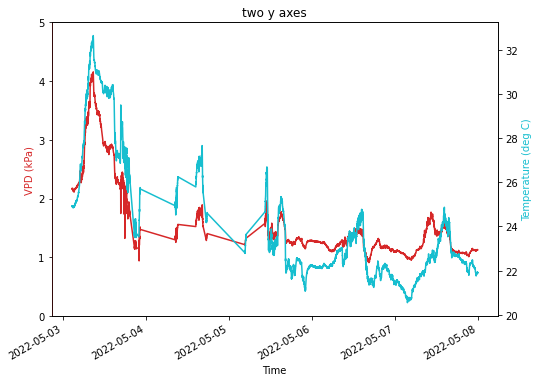
\includegraphics{introduction/first-steps_files/figure-pdf/cell-9-output-2.png}

}

\end{figure}

\hypertarget{nan-missing-data-outliers}{%
\section{NaN, Missing data, Outliers}\label{nan-missing-data-outliers}}

\begin{Shaded}
\begin{Highlighting}[]
\CommentTok{\# \%matplotlib widget}

\NormalTok{start }\OperatorTok{=} \StringTok{"2022{-}05{-}03 12:00:00"}
\NormalTok{end }\OperatorTok{=} \StringTok{"2022{-}05{-}06 00:00:00"}

\NormalTok{fig, ax }\OperatorTok{=}\NormalTok{ plt.subplots(}\DecValTok{1}\NormalTok{, figsize}\OperatorTok{=}\NormalTok{(}\DecValTok{8}\NormalTok{,}\DecValTok{4}\NormalTok{))}

\CommentTok{\# plot using pandas\textquotesingle{} plot method}
\NormalTok{df.loc[start:end, }\StringTok{\textquotesingle{}T2\textquotesingle{}}\NormalTok{].plot(ax}\OperatorTok{=}\NormalTok{ax,}
\NormalTok{                             linestyle}\OperatorTok{=}\StringTok{\textquotesingle{}{-}\textquotesingle{}}\NormalTok{,}
\NormalTok{                             marker}\OperatorTok{=}\StringTok{\textquotesingle{}o\textquotesingle{}}\NormalTok{,}
\NormalTok{                             color}\OperatorTok{=}\StringTok{"tab:blue"}\NormalTok{,}
\NormalTok{                             label}\OperatorTok{=}\StringTok{"data"}\NormalTok{)}

\CommentTok{\# annotate examples here:}
\CommentTok{\# https://jakevdp.github.io/PythonDataScienceHandbook/04.09{-}text{-}and{-}annotation.html}
\NormalTok{ax.annotate(}\StringTok{"NaN"}\NormalTok{,                             }\CommentTok{\# text to write, if nothing, then ""}
\NormalTok{            xy}\OperatorTok{=}\NormalTok{(}\StringTok{\textquotesingle{}2022{-}05{-}03 20:30:00\textquotesingle{}}\NormalTok{, }\DecValTok{25}\NormalTok{),    }\CommentTok{\# (x,y coordinates for the tip of the arrow)}
\NormalTok{            xycoords}\OperatorTok{=}\StringTok{\textquotesingle{}data\textquotesingle{}}\NormalTok{,                   }\CommentTok{\# xy as \textquotesingle{}data\textquotesingle{} coordinates}
\NormalTok{            xytext}\OperatorTok{=}\NormalTok{(}\OperatorTok{{-}}\DecValTok{20}\NormalTok{, }\DecValTok{60}\NormalTok{),                  }\CommentTok{\# xy coordinates for the text}
\NormalTok{            textcoords}\OperatorTok{=}\StringTok{\textquotesingle{}offset points\textquotesingle{}}\NormalTok{,        }\CommentTok{\# xytext relative to xy}
\NormalTok{            arrowprops}\OperatorTok{=}\BuiltInTok{dict}\NormalTok{(arrowstyle}\OperatorTok{=}\StringTok{"{-}\textgreater{}"}\NormalTok{)   }\CommentTok{\# pretty arrow}
\NormalTok{           )}
\NormalTok{ax.annotate(}\StringTok{"outlier"}\NormalTok{,}
\NormalTok{            xy}\OperatorTok{=}\NormalTok{(}\StringTok{\textquotesingle{}2022{-}05{-}03 22:30:00\textquotesingle{}}\NormalTok{, }\DecValTok{85}\NormalTok{),}
\NormalTok{            xycoords}\OperatorTok{=}\StringTok{\textquotesingle{}data\textquotesingle{}}\NormalTok{,}
\NormalTok{            xytext}\OperatorTok{=}\NormalTok{(}\DecValTok{40}\NormalTok{, }\OperatorTok{{-}}\DecValTok{20}\NormalTok{),}
\NormalTok{            textcoords}\OperatorTok{=}\StringTok{\textquotesingle{}offset points\textquotesingle{}}\NormalTok{,}
\NormalTok{            arrowprops}\OperatorTok{=}\BuiltInTok{dict}\NormalTok{(arrowstyle}\OperatorTok{=}\StringTok{"{-}\textgreater{}"}\NormalTok{)}
\NormalTok{           )}
\NormalTok{ax.annotate(}\StringTok{"missing rows"}\NormalTok{,}
\NormalTok{            xy}\OperatorTok{=}\NormalTok{(}\StringTok{\textquotesingle{}2022{-}05{-}05 00:00:00\textquotesingle{}}\NormalTok{, }\DecValTok{25}\NormalTok{),}
\NormalTok{            xycoords}\OperatorTok{=}\StringTok{\textquotesingle{}data\textquotesingle{}}\NormalTok{,}
\NormalTok{            xytext}\OperatorTok{=}\NormalTok{(}\DecValTok{0}\NormalTok{, }\DecValTok{40}\NormalTok{),}
\NormalTok{            textcoords}\OperatorTok{=}\StringTok{\textquotesingle{}offset points\textquotesingle{}}\NormalTok{,}
\NormalTok{            arrowprops}\OperatorTok{=}\BuiltInTok{dict}\NormalTok{(arrowstyle}\OperatorTok{=}\StringTok{"{-}\textgreater{}"}\NormalTok{)}
\NormalTok{           )}

\NormalTok{ax.xaxis.set\_major\_formatter(mdates.DateFormatter(}\StringTok{\textquotesingle{}}\SpecialCharTok{\%d}\StringTok{ \%b, \%H:00\textquotesingle{}}\NormalTok{))}
\NormalTok{plt.gcf().autofmt\_xdate()}
\NormalTok{ax.}\BuiltInTok{set}\NormalTok{(xlabel}\OperatorTok{=}\StringTok{""}\NormalTok{,}
\NormalTok{       ylabel}\OperatorTok{=}\StringTok{"Temperature (deg C)"}\NormalTok{)}
\end{Highlighting}
\end{Shaded}

\begin{verbatim}
[Text(0.5, 0, ''), Text(0, 0.5, 'Temperature (deg C)')]
\end{verbatim}

\begin{figure}[H]

{\centering 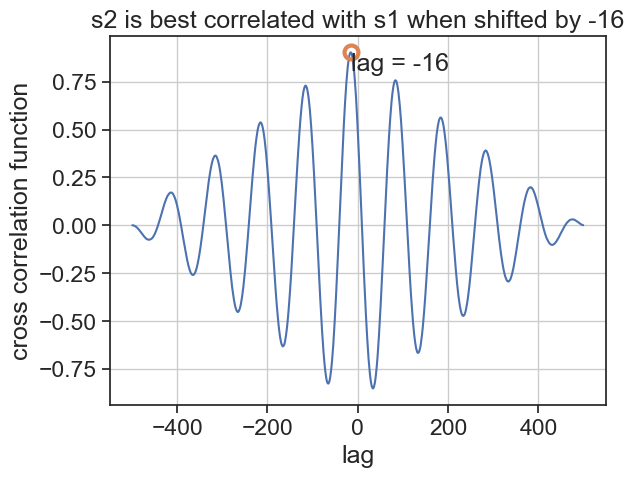
\includegraphics{introduction/first-steps_files/figure-pdf/cell-10-output-2.png}

}

\end{figure}

The arrows (annotate) work because the plot was\\
\texttt{df{[}\textquotesingle{}column\textquotesingle{}{]}.plot()}

If you use the usual\\
\texttt{ax.plot(df{[}\textquotesingle{}column\textquotesingle{}{]})}\strut \\
then you matplotlib will not understand timestamps as x-positions. In
this case follow the instructions below.

\begin{Shaded}
\begin{Highlighting}[]
\CommentTok{\# \%matplotlib widget}

\NormalTok{start }\OperatorTok{=} \StringTok{"2022{-}05{-}03 12:00:00"}
\NormalTok{end }\OperatorTok{=} \StringTok{"2022{-}05{-}06 00:00:00"}

\NormalTok{fig, ax }\OperatorTok{=}\NormalTok{ plt.subplots(}\DecValTok{1}\NormalTok{, figsize}\OperatorTok{=}\NormalTok{(}\DecValTok{8}\NormalTok{,}\DecValTok{4}\NormalTok{))}

\NormalTok{ax.plot(df.loc[start:end, }\StringTok{\textquotesingle{}T2\textquotesingle{}}\NormalTok{], linestyle}\OperatorTok{=}\StringTok{\textquotesingle{}{-}\textquotesingle{}}\NormalTok{, marker}\OperatorTok{=}\StringTok{\textquotesingle{}o\textquotesingle{}}\NormalTok{, color}\OperatorTok{=}\StringTok{"tab:blue"}\NormalTok{, label}\OperatorTok{=}\StringTok{"data"}\NormalTok{)}

\NormalTok{t\_nan }\OperatorTok{=} \StringTok{\textquotesingle{}2022{-}05{-}03 20:30:00\textquotesingle{}}
\NormalTok{x\_nan }\OperatorTok{=}\NormalTok{ mdates.date2num(dt.datetime.strptime(t\_nan, }\StringTok{"\%Y{-}\%m{-}}\SpecialCharTok{\%d}\StringTok{ \%H:\%M:\%S"}\NormalTok{))}
\NormalTok{ax.annotate(}\StringTok{"NaN"}\NormalTok{,}
\NormalTok{            xy}\OperatorTok{=}\NormalTok{(x\_nan, }\DecValTok{25}\NormalTok{),}
\NormalTok{            xycoords}\OperatorTok{=}\StringTok{\textquotesingle{}data\textquotesingle{}}\NormalTok{,}
\NormalTok{            xytext}\OperatorTok{=}\NormalTok{(}\OperatorTok{{-}}\DecValTok{20}\NormalTok{, }\DecValTok{60}\NormalTok{),}
\NormalTok{            textcoords}\OperatorTok{=}\StringTok{\textquotesingle{}offset points\textquotesingle{}}\NormalTok{,}
\NormalTok{            arrowprops}\OperatorTok{=}\BuiltInTok{dict}\NormalTok{(arrowstyle}\OperatorTok{=}\StringTok{"{-}\textgreater{}"}\NormalTok{)}
\NormalTok{           )}
\NormalTok{t\_outlier }\OperatorTok{=} \StringTok{\textquotesingle{}2022{-}05{-}03 22:30:00\textquotesingle{}}
\NormalTok{x\_outlier }\OperatorTok{=}\NormalTok{ mdates.date2num(dt.datetime.strptime(t\_outlier, }\StringTok{"\%Y{-}\%m{-}}\SpecialCharTok{\%d}\StringTok{ \%H:\%M:\%S"}\NormalTok{))}
\NormalTok{ax.annotate(}\StringTok{"outlier"}\NormalTok{,}
\NormalTok{            xy}\OperatorTok{=}\NormalTok{(x\_outlier, }\DecValTok{85}\NormalTok{),}
\NormalTok{            xycoords}\OperatorTok{=}\StringTok{\textquotesingle{}data\textquotesingle{}}\NormalTok{,}
\NormalTok{            xytext}\OperatorTok{=}\NormalTok{(}\DecValTok{40}\NormalTok{, }\OperatorTok{{-}}\DecValTok{20}\NormalTok{),}
\NormalTok{            textcoords}\OperatorTok{=}\StringTok{\textquotesingle{}offset points\textquotesingle{}}\NormalTok{,}
\NormalTok{            arrowprops}\OperatorTok{=}\BuiltInTok{dict}\NormalTok{(arrowstyle}\OperatorTok{=}\StringTok{"{-}\textgreater{}"}\NormalTok{)}
\NormalTok{           )}
\NormalTok{t\_missing }\OperatorTok{=} \StringTok{\textquotesingle{}2022{-}05{-}05 00:00:00\textquotesingle{}}
\NormalTok{x\_missing }\OperatorTok{=}\NormalTok{ mdates.date2num(dt.datetime.strptime(t\_missing, }\StringTok{"\%Y{-}\%m{-}}\SpecialCharTok{\%d}\StringTok{ \%H:\%M:\%S"}\NormalTok{))}
\NormalTok{ax.annotate(}\StringTok{"missing rows"}\NormalTok{,}
\NormalTok{            xy}\OperatorTok{=}\NormalTok{(x\_missing, }\DecValTok{25}\NormalTok{),}
\NormalTok{            xycoords}\OperatorTok{=}\StringTok{\textquotesingle{}data\textquotesingle{}}\NormalTok{,}
\NormalTok{            xytext}\OperatorTok{=}\NormalTok{(}\DecValTok{0}\NormalTok{, }\DecValTok{40}\NormalTok{),}
\NormalTok{            textcoords}\OperatorTok{=}\StringTok{\textquotesingle{}offset points\textquotesingle{}}\NormalTok{,}
\NormalTok{            arrowprops}\OperatorTok{=}\BuiltInTok{dict}\NormalTok{(arrowstyle}\OperatorTok{=}\StringTok{"{-}\textgreater{}"}\NormalTok{)}
\NormalTok{           )}
\CommentTok{\# code for hours, days, etc}
\CommentTok{\# https://docs.python.org/3/library/datetime.html\#strftime{-}and{-}strptime{-}format{-}codes}
\NormalTok{ax.xaxis.set\_major\_formatter(mdates.DateFormatter(}\StringTok{\textquotesingle{}}\SpecialCharTok{\%d}\StringTok{ \%b, \%H:00\textquotesingle{}}\NormalTok{))}
\NormalTok{plt.gcf().autofmt\_xdate()}
\NormalTok{ax.}\BuiltInTok{set}\NormalTok{(xlabel}\OperatorTok{=}\StringTok{""}\NormalTok{,}
\NormalTok{       ylabel}\OperatorTok{=}\StringTok{"Temperature (deg C)"}\NormalTok{)}
\end{Highlighting}
\end{Shaded}

\begin{verbatim}
[Text(0.5, 0, ''), Text(0, 0.5, 'Temperature (deg C)')]
\end{verbatim}

\begin{figure}[H]

{\centering 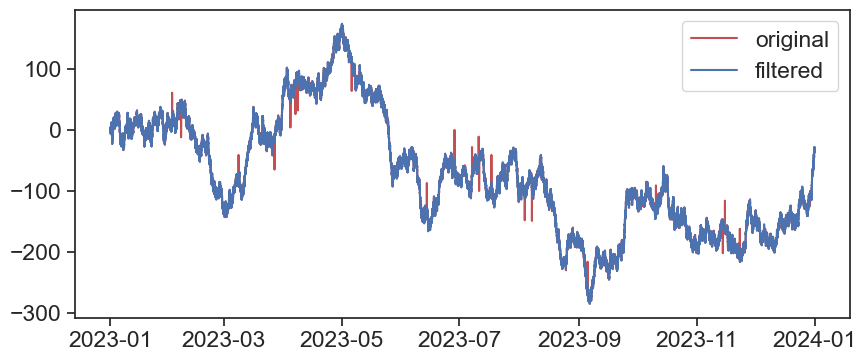
\includegraphics{introduction/first-steps_files/figure-pdf/cell-11-output-2.png}

}

\end{figure}

\begin{Shaded}
\begin{Highlighting}[]
\CommentTok{\# \%matplotlib widget}

\NormalTok{fig, ax }\OperatorTok{=}\NormalTok{ plt.subplots(}\DecValTok{1}\NormalTok{, figsize}\OperatorTok{=}\NormalTok{(}\DecValTok{8}\NormalTok{,}\DecValTok{4}\NormalTok{))}

\NormalTok{delta\_index }\OperatorTok{=}\NormalTok{ (df.index.to\_series().diff() }\OperatorTok{/}\NormalTok{ pd.Timedelta(}\StringTok{\textquotesingle{}1 sec\textquotesingle{}}\NormalTok{) ).values}
\NormalTok{ax.plot(delta\_index)}
\NormalTok{ax.}\BuiltInTok{set}\NormalTok{(ylim}\OperatorTok{=}\NormalTok{[}\DecValTok{0}\NormalTok{, }\DecValTok{100}\NormalTok{],}
\NormalTok{       xlabel}\OperatorTok{=}\StringTok{"running index"}\NormalTok{,}
\NormalTok{       ylabel}\OperatorTok{=}\VerbatimStringTok{r"$\textbackslash{}Delta t$ (s)"}\NormalTok{,}
\NormalTok{       title}\OperatorTok{=}\StringTok{"Time difference between consecutive rows"}\NormalTok{)}
\end{Highlighting}
\end{Shaded}

\begin{verbatim}
[(0.0, 100.0),
 Text(0.5, 0, 'running index'),
 Text(0, 0.5, '$\\Delta t$ (s)'),
 Text(0.5, 1.0, 'Time difference between consecutive rows')]
\end{verbatim}

\begin{figure}[H]

{\centering 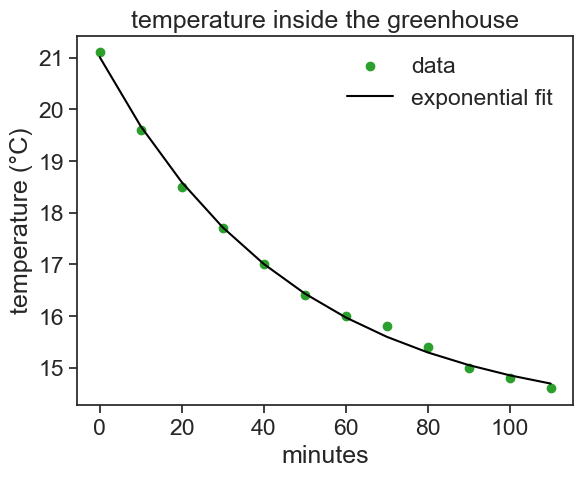
\includegraphics{introduction/first-steps_files/figure-pdf/cell-12-output-2.png}

}

\end{figure}

\hypertarget{resample}{%
\section{Resample}\label{resample}}

\hypertarget{downsampling}{%
\subsection{Downsampling}\label{downsampling}}

\begin{Shaded}
\begin{Highlighting}[]
\CommentTok{\# \%matplotlib widget}

\NormalTok{fig, ax }\OperatorTok{=}\NormalTok{ plt.subplots(}\DecValTok{1}\NormalTok{, figsize}\OperatorTok{=}\NormalTok{(}\DecValTok{8}\NormalTok{,}\DecValTok{4}\NormalTok{))}

\CommentTok{\# Downsample to spaced out data points. Change the number below, see what happens.}
\NormalTok{window\_size }\OperatorTok{=} \StringTok{\textquotesingle{}15min\textquotesingle{}}
\NormalTok{df\_resampled }\OperatorTok{=}\NormalTok{ (df[}\StringTok{\textquotesingle{}T2\textquotesingle{}}\NormalTok{].resample(window\_size)  }\CommentTok{\# resample doesn\textquotesingle{}t do anything yet, just divides data into buckets}
\NormalTok{                        .mean()                 }\CommentTok{\# this is where stuff happens. you can also choose "sum", "max", etc}
\NormalTok{               )}
\CommentTok{\# optional, add half a window size to timestamp}
\NormalTok{df\_resampled.index }\OperatorTok{=}\NormalTok{ df\_resampled.index }\OperatorTok{+}\NormalTok{ to\_offset(window\_size) }\OperatorTok{/} \DecValTok{2}

\NormalTok{ax.plot(df[}\StringTok{\textquotesingle{}T2\textquotesingle{}}\NormalTok{], color}\OperatorTok{=}\StringTok{"tab:blue"}\NormalTok{, label}\OperatorTok{=}\StringTok{"original data"}\NormalTok{)}
\NormalTok{ax.plot(df\_resampled, marker}\OperatorTok{=}\StringTok{\textquotesingle{}x\textquotesingle{}}\NormalTok{, color}\OperatorTok{=}\StringTok{"tab:orange"}\NormalTok{, zorder}\OperatorTok{={-}}\DecValTok{1}\NormalTok{,}
\NormalTok{        label}\OperatorTok{=}\SpecialStringTok{f"resampled }\SpecialCharTok{\{}\NormalTok{window\_size}\SpecialCharTok{\}}\SpecialStringTok{ data"}\NormalTok{)}
\NormalTok{ax.legend()}

\NormalTok{ax.}\BuiltInTok{set}\NormalTok{(xlabel}\OperatorTok{=}\StringTok{"time"}\NormalTok{,}
\NormalTok{       ylabel}\OperatorTok{=}\StringTok{"temperature (deg C)"}\NormalTok{)}
\end{Highlighting}
\end{Shaded}

\begin{verbatim}
[Text(0.5, 0, 'time'), Text(0, 0.5, 'temperature (deg C)')]
\end{verbatim}

\begin{figure}[H]

{\centering 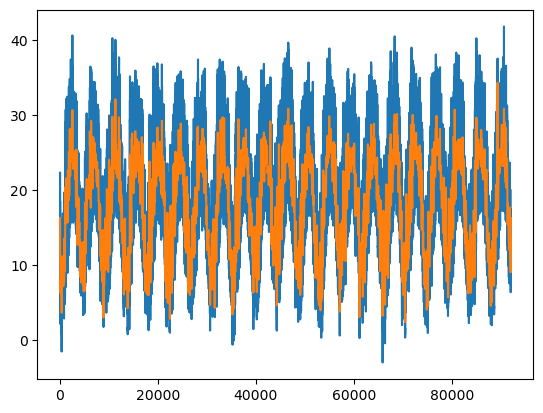
\includegraphics{introduction/first-steps_files/figure-pdf/cell-13-output-2.png}

}

\end{figure}

\hypertarget{filling-missing-data}{%
\subsection{Filling missing data}\label{filling-missing-data}}

\begin{Shaded}
\begin{Highlighting}[]
\CommentTok{\# \%matplotlib widget}

\NormalTok{fig, ax }\OperatorTok{=}\NormalTok{ plt.subplots(}\DecValTok{1}\NormalTok{, figsize}\OperatorTok{=}\NormalTok{(}\DecValTok{8}\NormalTok{,}\DecValTok{4}\NormalTok{))}

\CommentTok{\# see options for interpolation methods here:}
\CommentTok{\# https://pandas.pydata.org/docs/reference/api/pandas.DataFrame.interpolate.html}
\NormalTok{df\_interpolated1 }\OperatorTok{=}\NormalTok{ df\_resampled.interpolate(method}\OperatorTok{=}\StringTok{\textquotesingle{}time\textquotesingle{}}\NormalTok{)}
\NormalTok{df\_interpolated2 }\OperatorTok{=}\NormalTok{ df\_resampled.interpolate(method}\OperatorTok{=}\StringTok{\textquotesingle{}nearest\textquotesingle{}}\NormalTok{)}

\NormalTok{ax.plot(df\_resampled, color}\OperatorTok{=}\StringTok{"tab:orange"}\NormalTok{, label}\OperatorTok{=}\StringTok{"resampled"}\NormalTok{)}
\NormalTok{ax.plot(df\_interpolated1, }\StringTok{\textquotesingle{}.\textquotesingle{}}\NormalTok{, color}\OperatorTok{=}\StringTok{"tab:purple"}\NormalTok{, zorder}\OperatorTok{={-}}\DecValTok{1}\NormalTok{,}
\NormalTok{        label}\OperatorTok{=}\SpecialStringTok{f"time{-}interpolated"}\NormalTok{)}
\NormalTok{ax.plot(df\_interpolated2, }\StringTok{\textquotesingle{}.\textquotesingle{}}\NormalTok{, color}\OperatorTok{=}\StringTok{"tab:cyan"}\NormalTok{, zorder}\OperatorTok{={-}}\DecValTok{2}\NormalTok{,}
\NormalTok{        label}\OperatorTok{=}\SpecialStringTok{f"nearest{-}interpolated"}\NormalTok{)}
\NormalTok{ax.legend()}

\NormalTok{ax.}\BuiltInTok{set}\NormalTok{(xlabel}\OperatorTok{=}\StringTok{"time"}\NormalTok{,}
\NormalTok{       ylabel}\OperatorTok{=}\StringTok{"temperature (deg C)"}\NormalTok{)}
\end{Highlighting}
\end{Shaded}

\begin{verbatim}
[Text(0.5, 0, 'time'), Text(0, 0.5, 'temperature (deg C)')]
\end{verbatim}

\begin{figure}[H]

{\centering 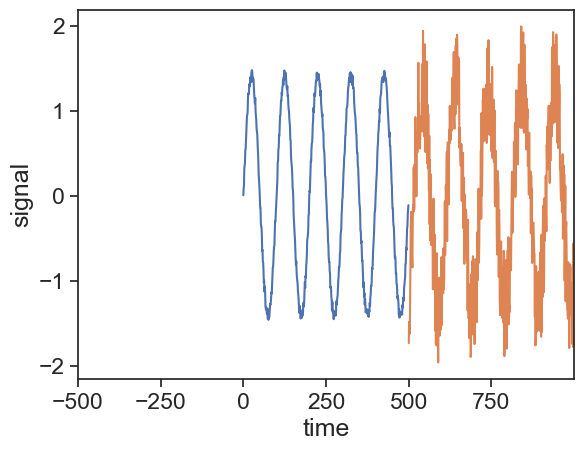
\includegraphics{introduction/first-steps_files/figure-pdf/cell-14-output-2.png}

}

\end{figure}

\hypertarget{smoothing-noisy-data}{%
\section{Smoothing noisy data}\label{smoothing-noisy-data}}

Let's first download data from a different project.

\begin{Shaded}
\begin{Highlighting}[]
\NormalTok{filename2 }\OperatorTok{=} \StringTok{"test\_peleg.csv"}
\CommentTok{\# if file is not there, go fetch it from thingspeak}
\ControlFlowTok{if} \KeywordTok{not}\NormalTok{ os.path.isfile(filename2):}
    \CommentTok{\# define what to download}
\NormalTok{    channels }\OperatorTok{=} \StringTok{"1708067"}
\NormalTok{    fields }\OperatorTok{=} \StringTok{"1,2,3,4,5"}
\NormalTok{    minutes }\OperatorTok{=} \StringTok{"30"}

    \CommentTok{\# https://www.mathworks.com/help/thingspeak/readdata.html}
    \CommentTok{\# format YYYY{-}MM{-}DD\%20HH:NN:SS}
\NormalTok{    start }\OperatorTok{=} \StringTok{"2022{-}05{-}15\%2000:00:00"}
\NormalTok{    end }\OperatorTok{=} \StringTok{"2022{-}05{-}25\%2000:00:00"}

    \CommentTok{\# download using Thingspeak\textquotesingle{}s API}
    \CommentTok{\# url = f"https://api.thingspeak.com/channels/\{channels\}/fields/\{fields\}.csv?minutes=\{minutes\}"}
\NormalTok{    url }\OperatorTok{=} \SpecialStringTok{f"https://api.thingspeak.com/channels/}\SpecialCharTok{\{}\NormalTok{channels}\SpecialCharTok{\}}\SpecialStringTok{/fields/}\SpecialCharTok{\{}\NormalTok{fields}\SpecialCharTok{\}}\SpecialStringTok{.csv?start=}\SpecialCharTok{\{}\NormalTok{start}\SpecialCharTok{\}}\SpecialStringTok{\&end=}\SpecialCharTok{\{}\NormalTok{end}\SpecialCharTok{\}}\SpecialStringTok{"}
\NormalTok{    data }\OperatorTok{=}\NormalTok{ urllib.request.urlopen(url)}
\NormalTok{    d }\OperatorTok{=}\NormalTok{ data.read()}

    \CommentTok{\# save data to csv}
    \BuiltInTok{file} \OperatorTok{=} \BuiltInTok{open}\NormalTok{(filename2, }\StringTok{"w"}\NormalTok{)}
    \BuiltInTok{file}\NormalTok{.write(d.decode(}\StringTok{\textquotesingle{}UTF{-}8\textquotesingle{}}\NormalTok{))}
    \BuiltInTok{file}\NormalTok{.close()}
\end{Highlighting}
\end{Shaded}

\begin{Shaded}
\begin{Highlighting}[]
\CommentTok{\# load data}
\NormalTok{df }\OperatorTok{=}\NormalTok{ pd.read\_csv(filename2)}
\CommentTok{\# rename columns}
\NormalTok{df }\OperatorTok{=}\NormalTok{ df.rename(columns}\OperatorTok{=}\NormalTok{\{}\StringTok{"created\_at"}\NormalTok{: }\StringTok{"timestamp"}\NormalTok{,}
                        \StringTok{"field1"}\NormalTok{: }\StringTok{"T"}\NormalTok{,}
                        \StringTok{"field2"}\NormalTok{: }\StringTok{"Tw"}\NormalTok{,}
                        \StringTok{"field3"}\NormalTok{: }\StringTok{"RH"}\NormalTok{,}
                        \StringTok{"field4"}\NormalTok{: }\StringTok{"VPD"}\NormalTok{,}
                        \StringTok{"field5"}\NormalTok{: }\StringTok{"dist"}\NormalTok{,}
\NormalTok{                        \})}
\CommentTok{\# set timestamp as index}
\NormalTok{df[}\StringTok{\textquotesingle{}timestamp\textquotesingle{}}\NormalTok{] }\OperatorTok{=}\NormalTok{ pd.to\_datetime(df[}\StringTok{\textquotesingle{}timestamp\textquotesingle{}}\NormalTok{])}
\NormalTok{df }\OperatorTok{=}\NormalTok{ df.set\_index(}\StringTok{\textquotesingle{}timestamp\textquotesingle{}}\NormalTok{)}
\end{Highlighting}
\end{Shaded}

\begin{Shaded}
\begin{Highlighting}[]
\NormalTok{df}
\end{Highlighting}
\end{Shaded}

\begin{longtable}[]{@{}lllllll@{}}
\toprule()
& entry\_id & T & Tw & RH & VPD & dist \\
timestamp & & & & & & \\
\midrule()
\endhead
2022-05-18 20:09:31+00:00 & 24716 & 23.85 & 23.3125 & 65.32 & 1.02532 &
7.208 \\
2022-05-18 20:10:32+00:00 & 24717 & 23.88 & 23.2500 & 65.32 & 1.02717 &
7.208 \\
2022-05-18 20:11:33+00:00 & 24718 & 23.90 & 23.2500 & 65.23 & 1.03107 &
7.276 \\
2022-05-18 20:12:33+00:00 & 24719 & 23.90 & 23.2500 & 65.19 & 1.03226 &
7.208 \\
2022-05-18 20:13:34+00:00 & 24720 & 23.89 & 23.2500 & 65.15 & 1.03282 &
7.633 \\
... & ... & ... & ... & ... & ... & ... \\
2022-05-24 12:18:35+00:00 & 32711 & 27.47 & 26.1250 & 47.49 & 1.92397 &
8.925 \\
2022-05-24 12:19:36+00:00 & 32712 & 27.47 & 26.1250 & 47.62 & 1.91921 &
8.925 \\
2022-05-24 12:20:39+00:00 & 32713 & 27.47 & 26.1250 & 47.96 & 1.90675 &
8.925 \\
2022-05-24 12:21:40+00:00 & 32714 & 27.47 & 26.1875 & 47.75 & 1.91444 &
8.925 \\
2022-05-24 12:22:41+00:00 & 32715 & 27.49 & 26.1875 & 47.94 & 1.90971 &
8.925 \\
\bottomrule()
\end{longtable}

\hypertarget{smoothing-noisy-data-1}{%
\section{Smoothing noisy data}\label{smoothing-noisy-data-1}}

\begin{Shaded}
\begin{Highlighting}[]
\CommentTok{\# \%matplotlib widget}

\NormalTok{fig, ax }\OperatorTok{=}\NormalTok{ plt.subplots(}\DecValTok{1}\NormalTok{, figsize}\OperatorTok{=}\NormalTok{(}\DecValTok{8}\NormalTok{,}\DecValTok{4}\NormalTok{))}

\NormalTok{ax.plot(df[}\StringTok{\textquotesingle{}RH\textquotesingle{}}\NormalTok{], }\StringTok{\textquotesingle{}.\textquotesingle{}}\NormalTok{)}
\CommentTok{\# add labels and title}
\NormalTok{ax.}\BuiltInTok{set}\NormalTok{(xlabel }\OperatorTok{=} \StringTok{"time"}\NormalTok{,}
\NormalTok{       ylabel }\OperatorTok{=} \StringTok{"RH (\%)"}\NormalTok{,}
\NormalTok{       title }\OperatorTok{=} \StringTok{"Relative Humidity"}\NormalTok{)}
\CommentTok{\# makes slanted dates}
\NormalTok{plt.gcf().autofmt\_xdate()  }
\end{Highlighting}
\end{Shaded}

\begin{figure}[H]

{\centering 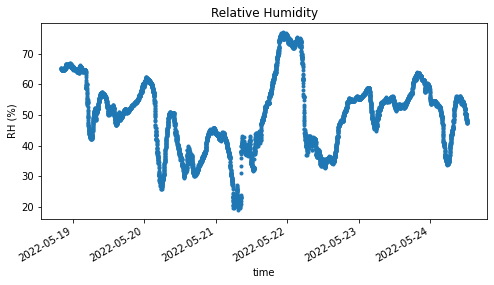
\includegraphics{introduction/first-steps_files/figure-pdf/cell-18-output-1.png}

}

\end{figure}

\hypertarget{moving-average-and-savgol}{%
\subsection{Moving average and SavGol}\label{moving-average-and-savgol}}

\begin{Shaded}
\begin{Highlighting}[]
\CommentTok{\# \%matplotlib widget}

\NormalTok{fig, ax }\OperatorTok{=}\NormalTok{ plt.subplots(}\DecValTok{1}\NormalTok{, figsize}\OperatorTok{=}\NormalTok{(}\DecValTok{8}\NormalTok{,}\DecValTok{4}\NormalTok{))}

\CommentTok{\# apply a rolling average of size "window\_size",}
\CommentTok{\# it can be either by number of points, or by window time}
\CommentTok{\# window\_size = 30  \# number of measurements}
\NormalTok{window\_size }\OperatorTok{=} \StringTok{\textquotesingle{}120min\textquotesingle{}}  \CommentTok{\# minutes}
\NormalTok{RH\_smooth }\OperatorTok{=}\NormalTok{ df[}\StringTok{\textquotesingle{}RH\textquotesingle{}}\NormalTok{].rolling(window\_size, center}\OperatorTok{=}\VariableTok{True}\NormalTok{).mean().to\_frame()}
\NormalTok{RH\_smooth.rename(columns}\OperatorTok{=}\NormalTok{\{}\StringTok{\textquotesingle{}RH\textquotesingle{}}\NormalTok{: }\StringTok{\textquotesingle{}rolling\_avg\textquotesingle{}}\NormalTok{\}, inplace}\OperatorTok{=}\VariableTok{True}\NormalTok{)}

\NormalTok{RH\_smooth[}\StringTok{\textquotesingle{}SG\textquotesingle{}}\NormalTok{] }\OperatorTok{=}\NormalTok{ savgol\_filter(df[}\StringTok{\textquotesingle{}RH\textquotesingle{}}\NormalTok{], window\_length}\OperatorTok{=}\DecValTok{121}\NormalTok{, polyorder}\OperatorTok{=}\DecValTok{2}\NormalTok{)}

\NormalTok{ax.plot(df[}\StringTok{\textquotesingle{}RH\textquotesingle{}}\NormalTok{], color}\OperatorTok{=}\StringTok{"tab:blue"}\NormalTok{, label}\OperatorTok{=}\StringTok{"data"}\NormalTok{)}
\NormalTok{ax.plot(RH\_smooth[}\StringTok{\textquotesingle{}rolling\_avg\textquotesingle{}}\NormalTok{], color}\OperatorTok{=}\StringTok{"tab:orange"}\NormalTok{, label}\OperatorTok{=}\StringTok{"moving average"}\NormalTok{)}
\NormalTok{ax.plot(RH\_smooth[}\StringTok{\textquotesingle{}SG\textquotesingle{}}\NormalTok{], color}\OperatorTok{=}\StringTok{"tab:red"}\NormalTok{, label}\OperatorTok{=}\StringTok{"Savitzky{-}Golay filter"}\NormalTok{)}
\CommentTok{\# add labels and title}
\NormalTok{ax.}\BuiltInTok{set}\NormalTok{(xlabel }\OperatorTok{=} \StringTok{"time"}\NormalTok{,}
\NormalTok{       ylabel }\OperatorTok{=} \StringTok{"RH (\%)"}\NormalTok{,}
\NormalTok{       title }\OperatorTok{=} \StringTok{"Relative Humidity"}\NormalTok{)}
\CommentTok{\# makes slanted dates}
\NormalTok{plt.gcf().autofmt\_xdate()}
\NormalTok{ax.legend()}
\end{Highlighting}
\end{Shaded}

\begin{verbatim}
<matplotlib.legend.Legend at 0x7fe6a0525730>
\end{verbatim}

\begin{figure}[H]

{\centering 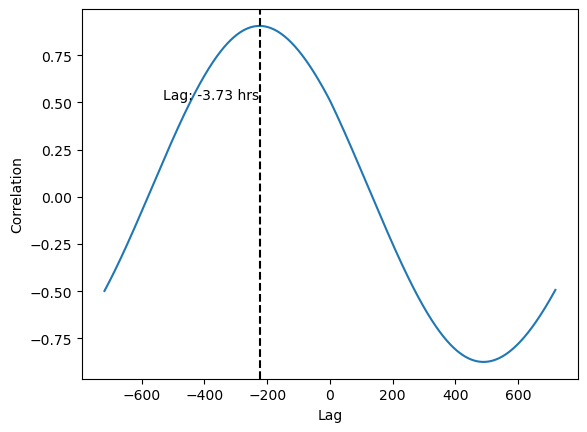
\includegraphics{introduction/first-steps_files/figure-pdf/cell-19-output-2.png}

}

\end{figure}

\part{Outliers and Gaps}

\hypertarget{z-score}{%
\chapter{Z-score}\label{z-score}}

\[
z  = \frac{x-\mu}{\sigma},
\]

\marginnote{\begin{footnotesize}

where

\begin{itemize}
\tightlist
\item
  \(x=\) data point,\\
\item
  \(\mu=\) time series mean\\
\item
  \(\sigma=\) time series standard deviation.
\end{itemize}

\end{footnotesize}}

Let's write a function that identifies outliers according to the
Z-score.

\begin{Shaded}
\begin{Highlighting}[]
\KeywordTok{def}\NormalTok{ zscore(df, degree}\OperatorTok{=}\DecValTok{3}\NormalTok{):}
\NormalTok{    data }\OperatorTok{=}\NormalTok{ df.copy()}
\NormalTok{    data[}\StringTok{\textquotesingle{}zscore\textquotesingle{}}\NormalTok{] }\OperatorTok{=}\NormalTok{ (data }\OperatorTok{{-}}\NormalTok{ data.mean())}\OperatorTok{/}\NormalTok{data.std()}
\NormalTok{    outliers }\OperatorTok{=}\NormalTok{ data[(data[}\StringTok{\textquotesingle{}zscore\textquotesingle{}}\NormalTok{] }\OperatorTok{\textless{}=} \OperatorTok{{-}}\NormalTok{degree) }\OperatorTok{|}\NormalTok{ (data[}\StringTok{\textquotesingle{}zscore\textquotesingle{}}\NormalTok{] }\OperatorTok{\textgreater{}=}\NormalTok{ degree)]}
    \ControlFlowTok{return}\NormalTok{ outliers[}\StringTok{\textquotesingle{}value\textquotesingle{}}\NormalTok{], data}
\end{Highlighting}
\end{Shaded}

Now we can simply use this function:

\begin{Shaded}
\begin{Highlighting}[]
\NormalTok{threshold }\OperatorTok{=} \FloatTok{2.5}
\NormalTok{outliers, transformed }\OperatorTok{=}\NormalTok{ zscore(tx, threshold)}
\end{Highlighting}
\end{Shaded}

Source: Atwan (2022)

\part{Resampling}

\hypertarget{upsampling-interpolation}{%
\chapter{Upsampling, interpolation}\label{upsampling-interpolation}}

\hypertarget{downsampling-1}{%
\chapter{Downsampling}\label{downsampling-1}}

\part{Best practices}

\hypertarget{dates}{%
\chapter{Dates}\label{dates}}

\part{Smoothing}

\hypertarget{convolution}{%
\chapter{Convolution}\label{convolution}}

Running windows of different shapes (kernels)

\hfill\break

This is the temperature for Tel Aviv, between 2 and 5 of January 2022.
Data is in intervals of 10 minutes, and was downloaded from the Israel
Meteorological Service.

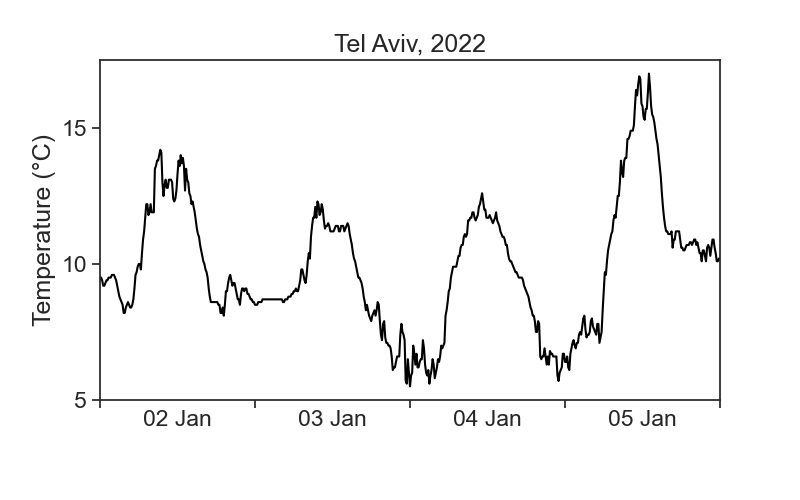
\includegraphics{smoothing/convolution_TA_temperature_2022.png}

We see that the temperature curve has a rough profile. Can we find ways
of getting smoother curves?

Convolution is a fancy word for averaging a time series using a running
window. We will use the terms \textbf{convolution, running average, and
rolling average} interchangeably. See the animation below. We take all
temperature values inside a window of width 500 minutes (51 points), and
average them with equal weights. The weights profile is called
\texttt{kernel}.

The pink curve is much smoother than the original! However, the running
average cannot describe sharp temperature changes. If we decrease the
window width to 200 minutes (21 points), we get the following result.

There is a tradeoff between the smoothness of a curve, and its ability
to describe sharp temporal changes.

\hypertarget{kernels}{%
\section{Kernels}\label{kernels}}

We can modify our running average, so that values closer to the center
of the window have higher weights, and those further away count less.
This is achieved by changing the weight profile, or the shape of the
kernel. We see below the result of a running average using a triangular
window of base 500 minutes (51 points).

Things can get as fancy as we want. Instead of a triangular kernel,
which has sharp edges, we can choose a smoother gaussian kernel, see the
difference below. We used a gaussian kernel with 60-minute standard
deviation (the window in the animation is 4 standard deviations wide).

\hypertarget{math}{%
\section{Math}\label{math}}

The definition of a convolution between signal \(f(t)\) and kernel
\(k(t)\) is

\[
(f * k)(t) = \int f(\tau)k(t-\tau)d\tau.
\]

The expression \(f*k\) denotes the convolution of these two functions.
The argument of \(k\) is \(t-\tau\), meaning that the kernel runs from
left to right (as \(t\) does), and at every point the two signals (\(f\)
and \(k\)) are multiplied together. It is the product of the signal with
the weight function \(k\) that gives us an average. Because of
\(-\tau\), the kernel is flipped backwards, but this has no effect to
symmetric kernels, like to ones in the examples above. Finally, the
actual running average is not the convolution, but

\[
\frac{(f * k)(t)}{\displaystyle \int k(t)dt}.
\]

Whenever the integral of the kernel is 1, then the convolution will be
identical with the running average.

\hypertarget{numerics}{%
\section{Numerics}\label{numerics}}

Running averages are very common tools in time-series analysis. The
\texttt{pandas} package makes life quite simple. For example, in order
to calculate the running average of temperature using a rectangular
kernel, one writes

\begin{Shaded}
\begin{Highlighting}[]
\NormalTok{df[}\StringTok{\textquotesingle{}temperature\textquotesingle{}}\NormalTok{].rolling(window}\OperatorTok{=}\StringTok{\textquotesingle{}20\textquotesingle{}}\NormalTok{, center}\OperatorTok{=}\VariableTok{True}\NormalTok{).mean()}
\end{Highlighting}
\end{Shaded}

\begin{itemize}
\tightlist
\item
  \texttt{window=20} means that the width of the window is 20 points.
  Pandas lets us define a window width in time units, for example,
  \texttt{window=\textquotesingle{}120min\textquotesingle{}}.
\item
  \texttt{center=True} is needed in order to assign the result of
  averaging to the center of the window. Make it \texttt{False} and see
  what happens.
\item
  \texttt{mean()} is the actual calculation, the average of temperature
  over the window. The \texttt{rolling} part does not compute anything,
  it just creates a moving window, and we are free to calculate whatever
  we want. Try to calculate the standard deviation or the maximum, for
  example.
\end{itemize}

It is implicit in the command above a ``rectangular'' kernel. What if we
want other shapes?

\hypertarget{gaussian}{%
\subsection{Gaussian}\label{gaussian}}

\begin{Shaded}
\begin{Highlighting}[]
\NormalTok{(}
\NormalTok{df[}\StringTok{\textquotesingle{}temperature\textquotesingle{}}\NormalTok{].rolling(window}\OperatorTok{=}\NormalTok{window\_width,}
\NormalTok{                          center}\OperatorTok{=}\VariableTok{True}\NormalTok{,}
\NormalTok{                          win\_type}\OperatorTok{=}\StringTok{"gaussian"}\NormalTok{)}
\NormalTok{                 .mean(std}\OperatorTok{=}\NormalTok{std\_gaussian)}
\NormalTok{)}
\end{Highlighting}
\end{Shaded}

where * \texttt{window\_width} is an integer, number of points in your
window * \texttt{std\_gaussian} is the standard deviation of your
gaussian, measured in sample points, not time!

For instance, if we have measurements every 10 minutes, and our window
width is 500 minutes, then \texttt{window\_width\ =\ 500/10\ +\ 1}
(first and last included). If we want a standard deviation of 60
minutes, then \texttt{std\_gaussian\ =\ 6}. The gaussian kernel will
look like this:

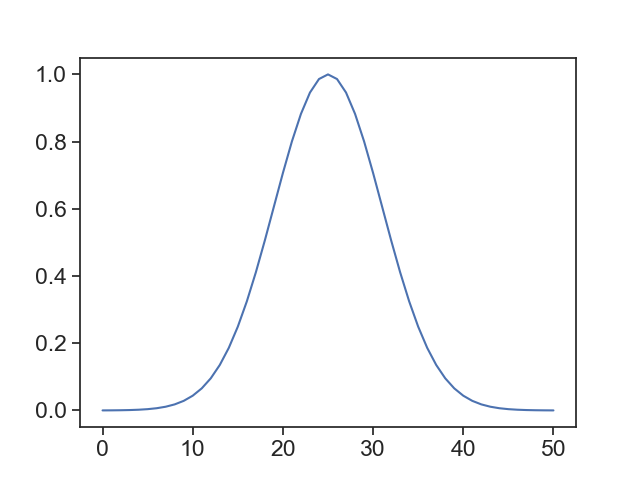
\includegraphics{smoothing/gaussian_kernel.png}

You can take a look at various options for kernel shapes
\href{https://docs.scipy.org/doc/scipy/reference/signal.windows.html\#module-scipy.signal.windows}{here},
provided by the \texttt{scipy} package. The graph above was achieved by
running:

\begin{Shaded}
\begin{Highlighting}[]
\NormalTok{g }\OperatorTok{=}\NormalTok{ scipy.signal.gaussian(window\_width, std)}
\NormalTok{plt.plot(g)}
\end{Highlighting}
\end{Shaded}

\hypertarget{triangular}{%
\subsection{Triangular}\label{triangular}}

Same idea as gaussian, but simpler, because we don't need to think about
standard deviation.

\begin{Shaded}
\begin{Highlighting}[]
\NormalTok{(}
\NormalTok{df[}\StringTok{\textquotesingle{}temperature\textquotesingle{}}\NormalTok{].rolling(window}\OperatorTok{=}\NormalTok{window\_width,}
\NormalTok{                          center}\OperatorTok{=}\VariableTok{True}\NormalTok{,}
\NormalTok{                          win\_type}\OperatorTok{=}\StringTok{"triang"}\NormalTok{)}
\NormalTok{                 .mean()}
\NormalTok{)}
\end{Highlighting}
\end{Shaded}

\hypertarget{which-window-shape-and-width-to-choose}{%
\section{🤷‍♂️ Which window shape and width to
choose?}\label{which-window-shape-and-width-to-choose}}

Sorry, there is not definite answer here\ldots{} It really depends on
your data and what you need to do with it. See below a comparison of all
examples in the videos above.

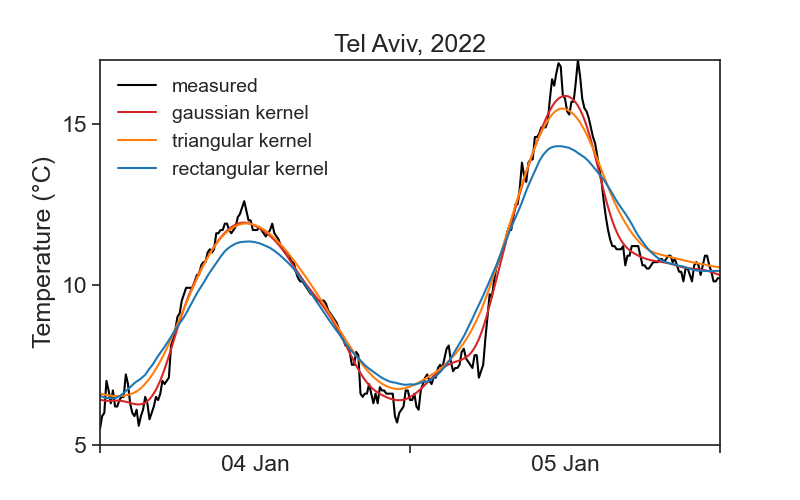
\includegraphics{smoothing/kernel_comparison.png}

\hypertarget{loess}{%
\chapter{LOESS}\label{loess}}

\hypertarget{a-perfect-smoother}{%
\chapter{A perfect smoother}\label{a-perfect-smoother}}

Source: Eilers (2003)

\href{https://github.com/mhvwerts/whittaker-eilers-smoother/tree/master}{GitHub
repository}

Noisy series \(y\) of length \(m\).

The smoothed series is called \(z\).

We have conflicting interests:

\begin{itemize}
\tightlist
\item
  we want a \(z\) series ``as smooth as possible''.
\item
  however, the smoother \(z\) is, the farthest from \(y\) it will be
  (low fidelity).
\end{itemize}

Roughness:

\[
R = \displaystyle\sum_i (z_i - z_{i-1})^2
\]

Fit to data:

\[
S = \displaystyle\sum_i (y_i - z_i)^2
\]

Cost functional to be minimized:

\[
Q = S + \lambda R
\]

\part{Stationarity}

\hypertarget{stochastic-processes}{%
\chapter{Stochastic processes}\label{stochastic-processes}}

\hypertarget{autocorrelation}{%
\chapter{Autocorrelation}\label{autocorrelation}}

See the temperatures for Jerusalem in a 4-day interval:

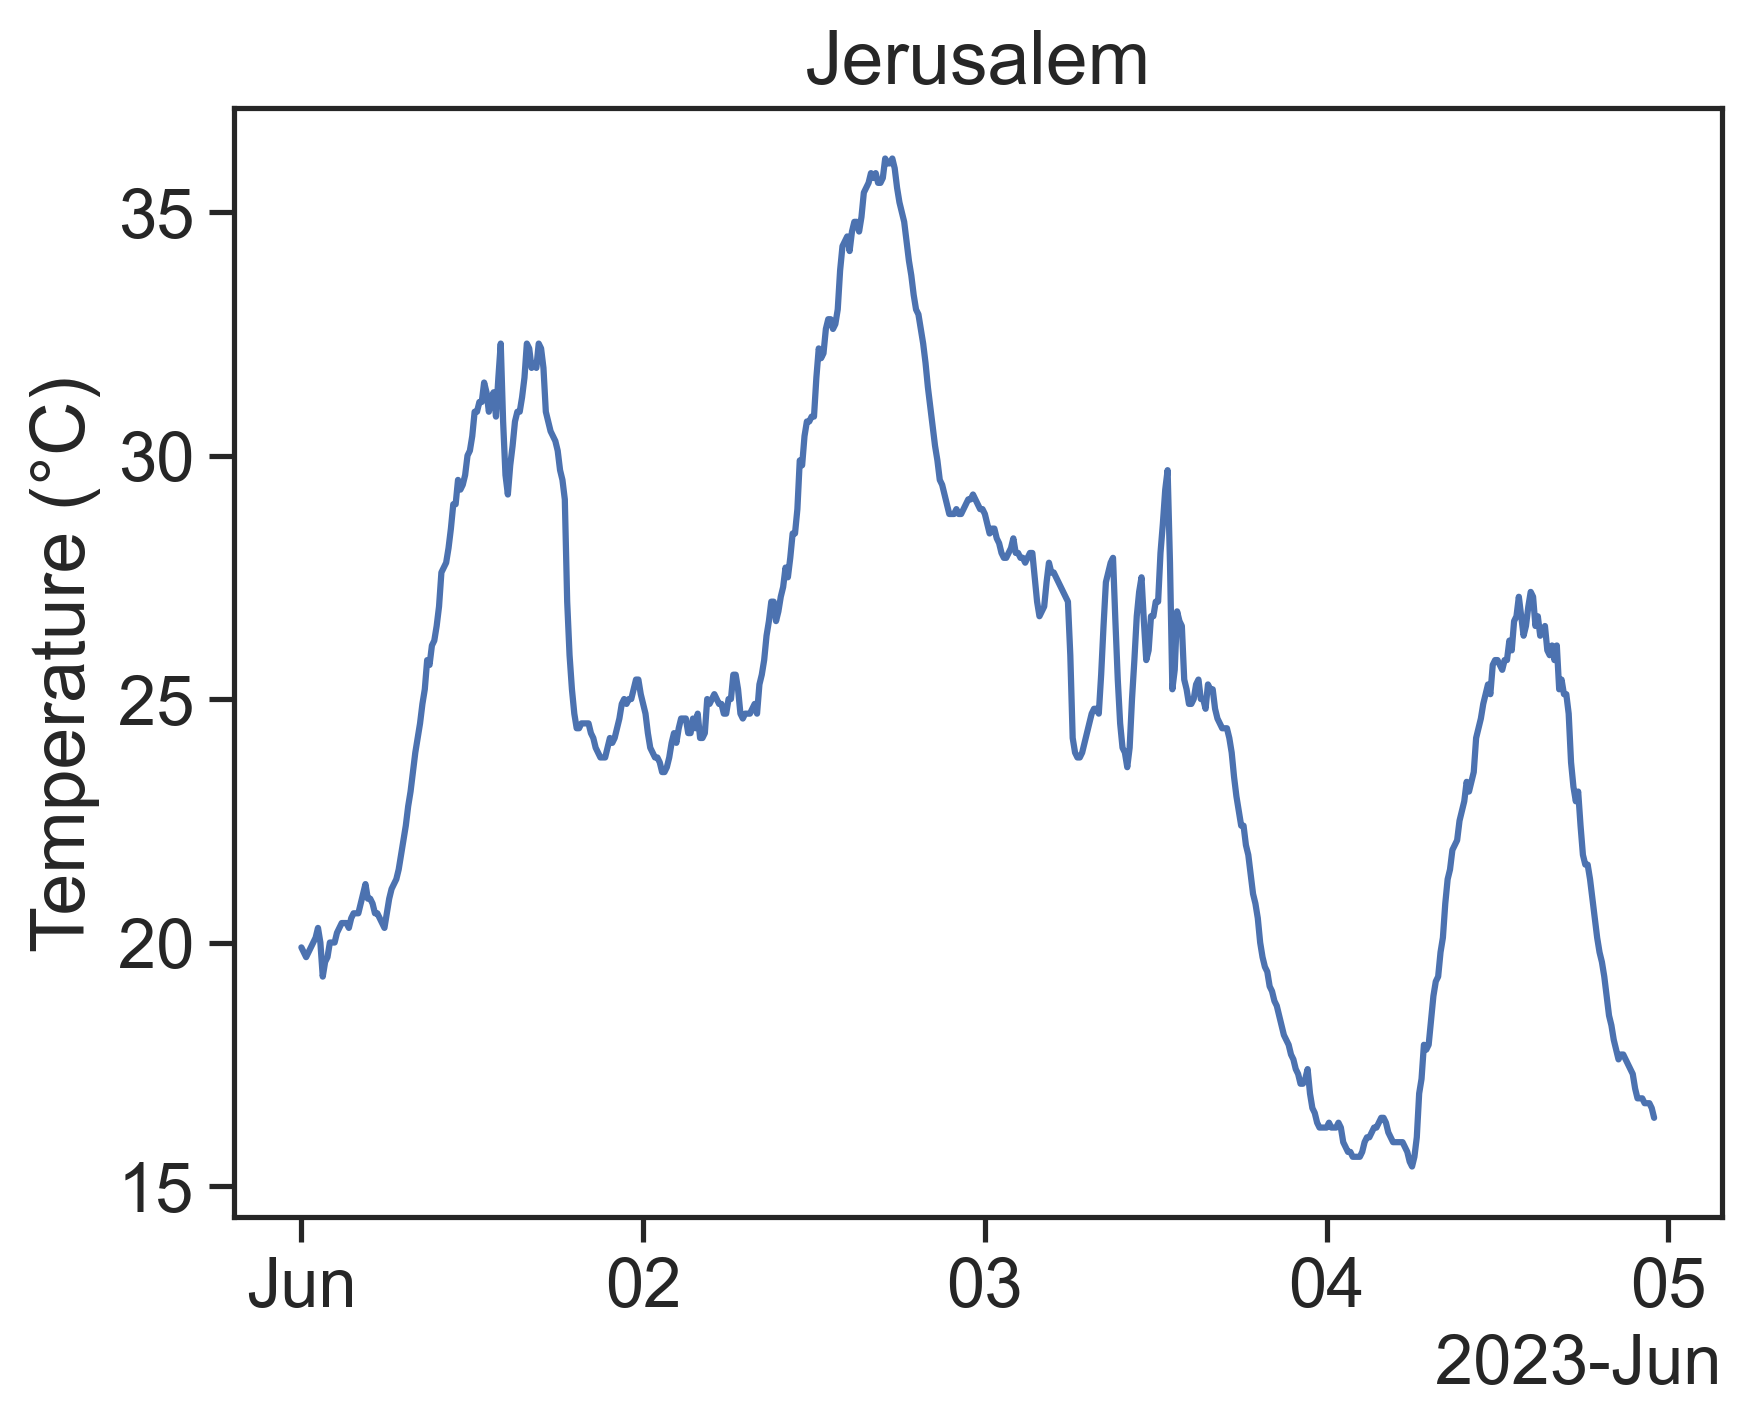
\includegraphics{stationarity/jer_temp1.png}

\hypertarget{question}{%
\section{Question}\label{question}}

If I know the temperature right now, what does that tell me about the
temperature 10 minutes from now? How about 100 minutes? 1000 minutes?

To answer this, we need to talk about \textbf{autocorrelation}. Let's
start by introducing the necessary concepts.

\hypertarget{mean-and-standard-deviation}{%
\section{Mean and standard
deviation}\label{mean-and-standard-deviation}}

Let's call our time series from above \(X\), and its length \(N\). Then:

\[
\begin{aligned}
\text{mean}& &\mu &= \frac{\displaystyle\sum_{i=1}^N X_i}{N} \\
\text{standard deviation}& &\sigma &= \sqrt{\frac{\displaystyle\sum_{i=1}^N (X_i-\mu)^2}{N}}
\end{aligned}
\]

The mean and standard deviation can be visualized thus:

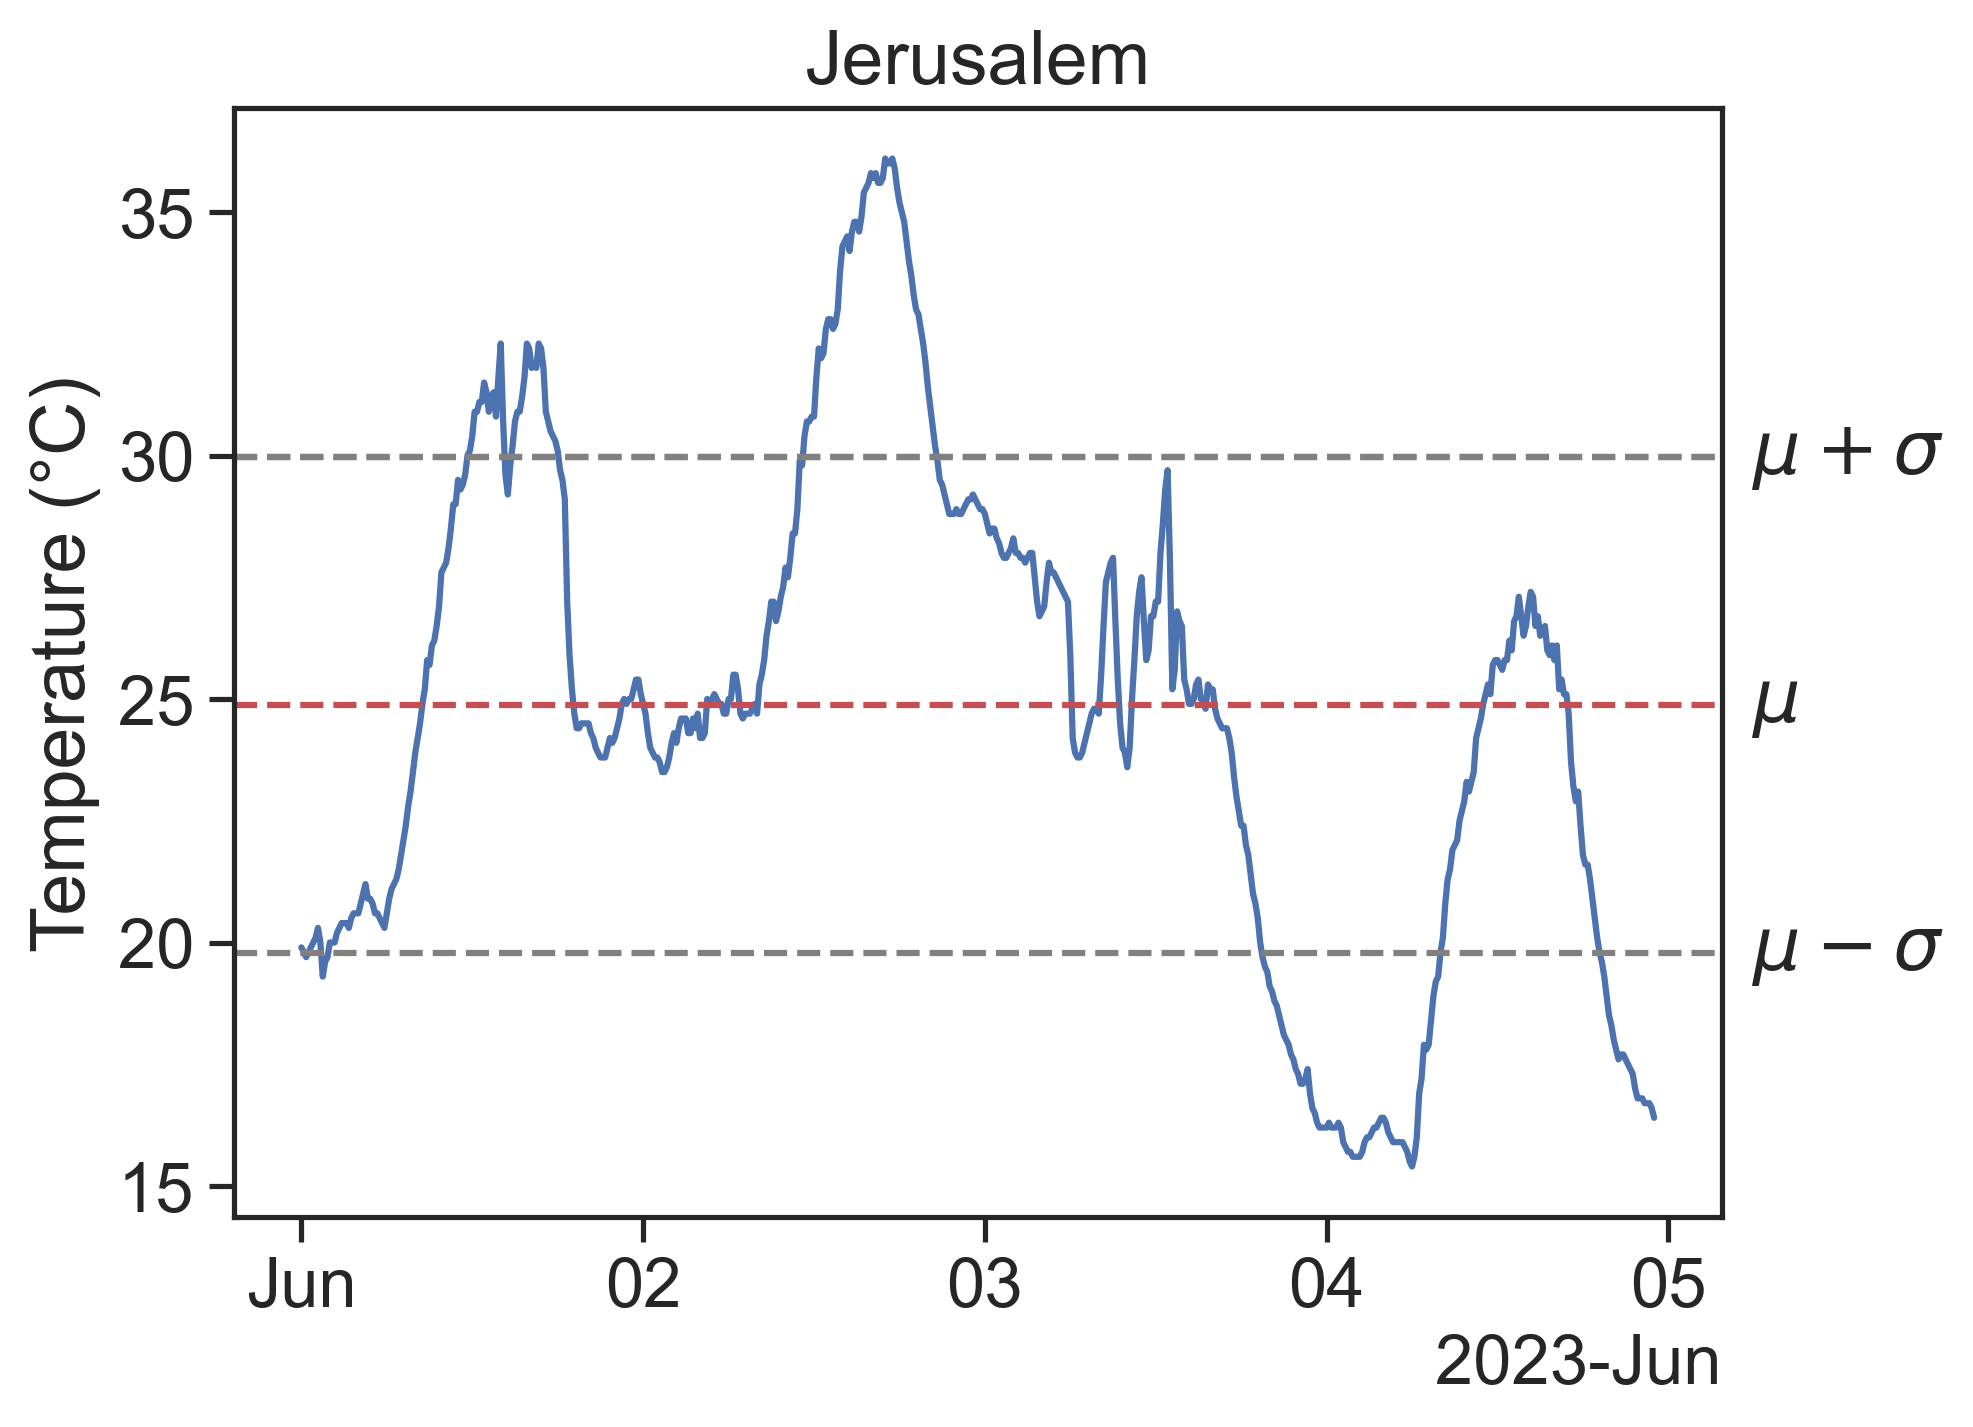
\includegraphics{stationarity/jer_temp2.png}

One last basic concept we need is the expected value: \[
E[X] = \sum_{i=1}^N X_i p_i
\]

For our time series, the probability \(p_i\) that a given point \(X_i\)
is in the dataset is simply \(1/N\), therefore the expectation becomes

\[
E[X] = \frac{\displaystyle\sum_{i=1}^N X_i}{N}
\]

\hypertarget{autocorrelation-1}{%
\section{Autocorrelation}\label{autocorrelation-1}}

The autocorrelation of a time series \(X\) is the answer to the
following question:

\begin{quote}
if we shift \(X\) by \(\tau\) units, how similar will this be to the
original signal?
\end{quote}

In other words:

\begin{quote}
how correlated are \(X(t)\) and \(X(t+\tau)\)?
\end{quote}

Using the Pearson correlation coefficient

\marginnote{\begin{footnotesize}

Pearson correlation coefficient between \(X\) and \(Y\): \[
\rho_{X,Y} = \frac{E\left[ (X - \mu_X)(X_Y - \mu_Y) \right]}{\sigma_X\sigma_Y}
\]

\end{footnotesize}}

we get

\[
\rho_{XX}(\tau) = \frac{E\left[ (X_t - \mu)(X_{t+\tau} - \mu) \right]}{\sigma^2}
\]

A video is worth a billion words, so let's see the autocorrelation in
action:

\url{https://youtu.be/tpf-tuYHR5w}

A few comments:

\begin{itemize}
\tightlist
\item
  The autocorrelation for \(\tau=0\) (zero shift) is always 1.\\
  {[}Can you prove this? All the necessary equations are above!{]}
\end{itemize}

\part{Time lags}

\hypertarget{cross-correlation}{%
\chapter{Cross-correlation}\label{cross-correlation}}

\begin{Shaded}
\begin{Highlighting}[]
\ImportTok{import}\NormalTok{ numpy }\ImportTok{as}\NormalTok{ np}
\end{Highlighting}
\end{Shaded}

\begin{Shaded}
\begin{Highlighting}[]
\BuiltInTok{print}\NormalTok{(}\StringTok{\textquotesingle{}dfvdfv\textquotesingle{}}\NormalTok{)}
\end{Highlighting}
\end{Shaded}

\begin{verbatim}
dfvdfv
\end{verbatim}

\hypertarget{dynamic-time-warp}{%
\chapter{Dynamic Time Warp}\label{dynamic-time-warp}}

\hypertarget{ldtw}{%
\chapter{LDTW}\label{ldtw}}

according to this paper

\part{Frequency}

\hypertarget{fourier-transform}{%
\chapter{Fourier transform}\label{fourier-transform}}

\hypertarget{filtering}{%
\chapter{Filtering}\label{filtering}}

\hypertarget{nyquist-shannon-sampling-theorem}{%
\chapter{Nyquist-Shannon sampling
theorem}\label{nyquist-shannon-sampling-theorem}}

\part{Seasonality}

\hypertarget{seasonal-decomposition}{%
\chapter{Seasonal Decomposition}\label{seasonal-decomposition}}

\begin{Shaded}
\begin{Highlighting}[]
\ImportTok{import}\NormalTok{ numpy }\ImportTok{as}\NormalTok{ np}
\ImportTok{import}\NormalTok{ matplotlib.pyplot }\ImportTok{as}\NormalTok{ plt}
\ImportTok{import}\NormalTok{ pandas }\ImportTok{as}\NormalTok{ pd}
\ImportTok{from}\NormalTok{ pandas.plotting }\ImportTok{import}\NormalTok{ register\_matplotlib\_converters}
\NormalTok{register\_matplotlib\_converters()  }\CommentTok{\# datetime converter for a matplotlib}
\ImportTok{import}\NormalTok{ seaborn }\ImportTok{as}\NormalTok{ sns}
\NormalTok{sns.}\BuiltInTok{set}\NormalTok{(style}\OperatorTok{=}\StringTok{"ticks"}\NormalTok{, font\_scale}\OperatorTok{=}\FloatTok{1.5}\NormalTok{)}
\ImportTok{from}\NormalTok{ statsmodels.tsa.seasonal }\ImportTok{import}\NormalTok{ seasonal\_decompose}
\ImportTok{import}\NormalTok{ matplotlib.dates }\ImportTok{as}\NormalTok{ mdates}
\ImportTok{from}\NormalTok{ matplotlib.dates }\ImportTok{import}\NormalTok{ DateFormatter}
\end{Highlighting}
\end{Shaded}

\hypertarget{trends-in-atmospheric-carbon-dioxide}{%
\chapter{Trends in Atmospheric Carbon
Dioxide}\label{trends-in-atmospheric-carbon-dioxide}}

Mauna Loa CO2 concentration.\\
data from \href{https://gml.noaa.gov/ccgg/trends/data.html}{NOAA}

\begin{Shaded}
\begin{Highlighting}[]
\NormalTok{url }\OperatorTok{=} \StringTok{"https://gml.noaa.gov/webdata/ccgg/trends/co2/co2\_weekly\_mlo.csv"}
\NormalTok{df }\OperatorTok{=}\NormalTok{ pd.read\_csv(url, header}\OperatorTok{=}\DecValTok{47}\NormalTok{, na\_values}\OperatorTok{=}\NormalTok{[}\OperatorTok{{-}}\FloatTok{999.99}\NormalTok{])}

\CommentTok{\# you can first download, and then read the csv}
\CommentTok{\# filename = "co2\_weekly\_mlo.csv"}
\CommentTok{\# df = pd.read\_csv(filename, header=47, na\_values=[{-}999.99])}

\NormalTok{df}
\end{Highlighting}
\end{Shaded}

\begin{longtable}[]{@{}llllllllll@{}}
\toprule()
& year & month & day & decimal & average & ndays & 1 year ago & 10 years
ago & increase since 1800 \\
\midrule()
\endhead
0 & 1974 & 5 & 19 & 1974.3795 & 333.37 & 5 & NaN & NaN & 50.40 \\
1 & 1974 & 5 & 26 & 1974.3986 & 332.95 & 6 & NaN & NaN & 50.06 \\
2 & 1974 & 6 & 2 & 1974.4178 & 332.35 & 5 & NaN & NaN & 49.60 \\
3 & 1974 & 6 & 9 & 1974.4370 & 332.20 & 7 & NaN & NaN & 49.65 \\
4 & 1974 & 6 & 16 & 1974.4562 & 332.37 & 7 & NaN & NaN & 50.06 \\
... & ... & ... & ... & ... & ... & ... & ... & ... & ... \\
2510 & 2022 & 6 & 26 & 2022.4836 & 420.31 & 7 & 418.14 & 395.36 &
138.71 \\
2511 & 2022 & 7 & 3 & 2022.5027 & 419.73 & 6 & 417.49 & 395.15 &
138.64 \\
2512 & 2022 & 7 & 10 & 2022.5219 & 419.08 & 6 & 417.25 & 394.59 &
138.52 \\
2513 & 2022 & 7 & 17 & 2022.5411 & 418.43 & 6 & 417.14 & 394.64 &
138.41 \\
2514 & 2022 & 7 & 24 & 2022.5603 & 417.84 & 6 & 415.68 & 394.11 &
138.36 \\
\bottomrule()
\end{longtable}

\begin{Shaded}
\begin{Highlighting}[]
\NormalTok{df[}\StringTok{\textquotesingle{}date\textquotesingle{}}\NormalTok{] }\OperatorTok{=}\NormalTok{ pd.to\_datetime(df[[}\StringTok{\textquotesingle{}year\textquotesingle{}}\NormalTok{, }\StringTok{\textquotesingle{}month\textquotesingle{}}\NormalTok{, }\StringTok{\textquotesingle{}day\textquotesingle{}}\NormalTok{]])}
\NormalTok{df }\OperatorTok{=}\NormalTok{ df.set\_index(}\StringTok{\textquotesingle{}date\textquotesingle{}}\NormalTok{)}
\NormalTok{df}
\end{Highlighting}
\end{Shaded}

\begin{longtable}[]{@{}llllllllll@{}}
\toprule()
& year & month & day & decimal & average & ndays & 1 year ago & 10 years
ago & increase since 1800 \\
date & & & & & & & & & \\
\midrule()
\endhead
1974-05-19 & 1974 & 5 & 19 & 1974.3795 & 333.37 & 5 & NaN & NaN &
50.40 \\
1974-05-26 & 1974 & 5 & 26 & 1974.3986 & 332.95 & 6 & NaN & NaN &
50.06 \\
1974-06-02 & 1974 & 6 & 2 & 1974.4178 & 332.35 & 5 & NaN & NaN &
49.60 \\
1974-06-09 & 1974 & 6 & 9 & 1974.4370 & 332.20 & 7 & NaN & NaN &
49.65 \\
1974-06-16 & 1974 & 6 & 16 & 1974.4562 & 332.37 & 7 & NaN & NaN &
50.06 \\
... & ... & ... & ... & ... & ... & ... & ... & ... & ... \\
2022-06-26 & 2022 & 6 & 26 & 2022.4836 & 420.31 & 7 & 418.14 & 395.36 &
138.71 \\
2022-07-03 & 2022 & 7 & 3 & 2022.5027 & 419.73 & 6 & 417.49 & 395.15 &
138.64 \\
2022-07-10 & 2022 & 7 & 10 & 2022.5219 & 419.08 & 6 & 417.25 & 394.59 &
138.52 \\
2022-07-17 & 2022 & 7 & 17 & 2022.5411 & 418.43 & 6 & 417.14 & 394.64 &
138.41 \\
2022-07-24 & 2022 & 7 & 24 & 2022.5603 & 417.84 & 6 & 415.68 & 394.11 &
138.36 \\
\bottomrule()
\end{longtable}

\begin{Shaded}
\begin{Highlighting}[]
\CommentTok{\# \%matplotlib widget}

\NormalTok{fig, ax }\OperatorTok{=}\NormalTok{ plt.subplots(}\DecValTok{1}\NormalTok{, figsize}\OperatorTok{=}\NormalTok{(}\DecValTok{8}\NormalTok{,}\DecValTok{6}\NormalTok{))}
\NormalTok{ax.plot(df[}\StringTok{\textquotesingle{}average\textquotesingle{}}\NormalTok{])}
\NormalTok{ax.}\BuiltInTok{set}\NormalTok{(xlabel}\OperatorTok{=}\StringTok{"date"}\NormalTok{,}
\NormalTok{       ylabel}\OperatorTok{=}\StringTok{"CO2 concentration (ppm)"}\NormalTok{,}
       \CommentTok{\# ylim=[0, 430],}
\NormalTok{       title}\OperatorTok{=}\StringTok{"Mauna Loa CO2 concentration"}\NormalTok{)}\OperatorTok{;}
\end{Highlighting}
\end{Shaded}

\begin{figure}[H]

{\centering \includegraphics{seasonality/seasonal-decomposition_files/figure-pdf/cell-5-output-1.png}

}

\end{figure}

fill missing data. interpolate method: `time'\\
\href{https://thepythonyouneed.com/how-to-interpolate-values-with-pandas/}{interpolation
methods visualized}

\begin{Shaded}
\begin{Highlighting}[]
\NormalTok{df[}\StringTok{\textquotesingle{}co2\textquotesingle{}}\NormalTok{] }\OperatorTok{=}\NormalTok{ (df[}\StringTok{\textquotesingle{}average\textquotesingle{}}\NormalTok{].resample(}\StringTok{"D"}\NormalTok{) }\CommentTok{\#resample daily}
\NormalTok{                          .interpolate(method}\OperatorTok{=}\StringTok{\textquotesingle{}time\textquotesingle{}}\NormalTok{) }\CommentTok{\#interpolate by time}
\NormalTok{            )}
\NormalTok{df}
\end{Highlighting}
\end{Shaded}

\begin{longtable}[]{@{}lllllllllll@{}}
\toprule()
& year & month & day & decimal & average & ndays & 1 year ago & 10 years
ago & increase since 1800 & co2 \\
date & & & & & & & & & & \\
\midrule()
\endhead
1974-05-19 & 1974 & 5 & 19 & 1974.3795 & 333.37 & 5 & NaN & NaN & 50.40
& 333.37 \\
1974-05-26 & 1974 & 5 & 26 & 1974.3986 & 332.95 & 6 & NaN & NaN & 50.06
& 332.95 \\
1974-06-02 & 1974 & 6 & 2 & 1974.4178 & 332.35 & 5 & NaN & NaN & 49.60 &
332.35 \\
1974-06-09 & 1974 & 6 & 9 & 1974.4370 & 332.20 & 7 & NaN & NaN & 49.65 &
332.20 \\
1974-06-16 & 1974 & 6 & 16 & 1974.4562 & 332.37 & 7 & NaN & NaN & 50.06
& 332.37 \\
... & ... & ... & ... & ... & ... & ... & ... & ... & ... & ... \\
2022-06-26 & 2022 & 6 & 26 & 2022.4836 & 420.31 & 7 & 418.14 & 395.36 &
138.71 & 420.31 \\
2022-07-03 & 2022 & 7 & 3 & 2022.5027 & 419.73 & 6 & 417.49 & 395.15 &
138.64 & 419.73 \\
2022-07-10 & 2022 & 7 & 10 & 2022.5219 & 419.08 & 6 & 417.25 & 394.59 &
138.52 & 419.08 \\
2022-07-17 & 2022 & 7 & 17 & 2022.5411 & 418.43 & 6 & 417.14 & 394.64 &
138.41 & 418.43 \\
2022-07-24 & 2022 & 7 & 24 & 2022.5603 & 417.84 & 6 & 415.68 & 394.11 &
138.36 & 417.84 \\
\bottomrule()
\end{longtable}

\hypertarget{decompose-data}{%
\section{decompose data}\label{decompose-data}}

\texttt{seasonal\_decompose} returns an object with four components:

\begin{itemize}
\tightlist
\item
  observed: \(Y(t)\)
\item
  trend: \(T(t)\)
\item
  seasonal: \(S(t)\)
\item
  resid: \(e(t)\)
\end{itemize}

Additive model: \[
Y(t) = T(t) + S(t) + e(t)
\]

Multiplicative model: \[
Y(t) = T(t) \times S(t) \times e(t)
\]

\hypertarget{interlude}{%
\subsubsection{Interlude}\label{interlude}}

learn how to use \texttt{zip} in a loop

\begin{Shaded}
\begin{Highlighting}[]
\NormalTok{letters }\OperatorTok{=}\NormalTok{ [}\StringTok{\textquotesingle{}a\textquotesingle{}}\NormalTok{, }\StringTok{\textquotesingle{}b\textquotesingle{}}\NormalTok{, }\StringTok{\textquotesingle{}c\textquotesingle{}}\NormalTok{, }\StringTok{\textquotesingle{}d\textquotesingle{}}\NormalTok{, }\StringTok{\textquotesingle{}e\textquotesingle{}}\NormalTok{]}
\NormalTok{numbers }\OperatorTok{=}\NormalTok{ [}\DecValTok{1}\NormalTok{, }\DecValTok{2}\NormalTok{, }\DecValTok{3}\NormalTok{, }\DecValTok{4}\NormalTok{, }\DecValTok{5}\NormalTok{]}
\CommentTok{\# zip let\textquotesingle{}s us iterate over to lists at the same time}
\ControlFlowTok{for}\NormalTok{ l, n }\KeywordTok{in} \BuiltInTok{zip}\NormalTok{(letters, numbers):}
    \BuiltInTok{print}\NormalTok{(}\SpecialStringTok{f"}\SpecialCharTok{\{}\NormalTok{l}\SpecialCharTok{\}}\SpecialStringTok{ = }\SpecialCharTok{\{}\NormalTok{n}\SpecialCharTok{\}}\SpecialStringTok{"}\NormalTok{)}
\end{Highlighting}
\end{Shaded}

\begin{verbatim}
a = 1
b = 2
c = 3
d = 4
e = 5
\end{verbatim}

Plot each component separately.

\begin{Shaded}
\begin{Highlighting}[]
\CommentTok{\# \%matplotlib widget}

\NormalTok{fig, ax }\OperatorTok{=}\NormalTok{ plt.subplots(}\DecValTok{4}\NormalTok{, }\DecValTok{1}\NormalTok{, figsize}\OperatorTok{=}\NormalTok{(}\DecValTok{8}\NormalTok{,}\DecValTok{6}\NormalTok{), sharex}\OperatorTok{=}\VariableTok{True}\NormalTok{)}
\NormalTok{decomposed\_m }\OperatorTok{=}\NormalTok{ seasonal\_decompose(df[}\StringTok{\textquotesingle{}co2\textquotesingle{}}\NormalTok{], model}\OperatorTok{=}\StringTok{\textquotesingle{}multiplicative\textquotesingle{}}\NormalTok{)}
\NormalTok{decomposed\_a }\OperatorTok{=}\NormalTok{ seasonal\_decompose(df[}\StringTok{\textquotesingle{}co2\textquotesingle{}}\NormalTok{], model}\OperatorTok{=}\StringTok{\textquotesingle{}additive\textquotesingle{}}\NormalTok{)}
\NormalTok{decomposed }\OperatorTok{=}\NormalTok{ decomposed\_m}
\NormalTok{pos }\OperatorTok{=}\NormalTok{ (}\FloatTok{0.5}\NormalTok{, }\FloatTok{0.9}\NormalTok{)}
\NormalTok{components }\OperatorTok{=}\NormalTok{[}\StringTok{"observed"}\NormalTok{, }\StringTok{"trend"}\NormalTok{, }\StringTok{"seasonal"}\NormalTok{, }\StringTok{"resid"}\NormalTok{]}
\NormalTok{colors }\OperatorTok{=}\NormalTok{ [}\StringTok{"tab:blue"}\NormalTok{, }\StringTok{"tab:orange"}\NormalTok{, }\StringTok{"tab:green"}\NormalTok{, }\StringTok{"tab:red"}\NormalTok{]}
\ControlFlowTok{for}\NormalTok{ axx, component, color }\KeywordTok{in} \BuiltInTok{zip}\NormalTok{(ax, components, colors):}
\NormalTok{    data }\OperatorTok{=} \BuiltInTok{getattr}\NormalTok{(decomposed, component)}
\NormalTok{    axx.plot(data, color}\OperatorTok{=}\NormalTok{color)}
\NormalTok{    axx.text(}\OperatorTok{*}\NormalTok{pos, component, bbox}\OperatorTok{=}\BuiltInTok{dict}\NormalTok{(facecolor}\OperatorTok{=}\StringTok{\textquotesingle{}white\textquotesingle{}}\NormalTok{, alpha}\OperatorTok{=}\FloatTok{0.8}\NormalTok{),}
\NormalTok{           transform}\OperatorTok{=}\NormalTok{axx.transAxes, ha}\OperatorTok{=}\StringTok{\textquotesingle{}center\textquotesingle{}}\NormalTok{, va}\OperatorTok{=}\StringTok{\textquotesingle{}top\textquotesingle{}}\NormalTok{)}
\end{Highlighting}
\end{Shaded}

\begin{figure}[H]

{\centering 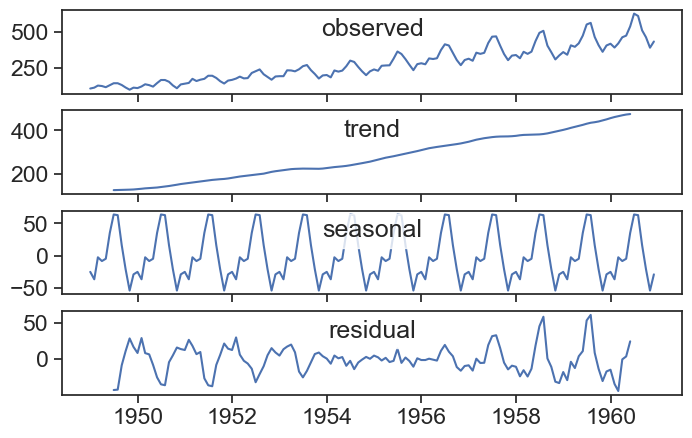
\includegraphics{seasonality/seasonal-decomposition_files/figure-pdf/cell-8-output-1.png}

}

\end{figure}

\begin{Shaded}
\begin{Highlighting}[]
\CommentTok{\# \%matplotlib widget}

\NormalTok{decomposed }\OperatorTok{=}\NormalTok{ decomposed\_m}

\NormalTok{fig, ax }\OperatorTok{=}\NormalTok{ plt.subplots(}\DecValTok{1}\NormalTok{, }\DecValTok{2}\NormalTok{, figsize}\OperatorTok{=}\NormalTok{(}\DecValTok{10}\NormalTok{,}\DecValTok{6}\NormalTok{))}
\NormalTok{ax[}\DecValTok{0}\NormalTok{].plot(df[}\StringTok{\textquotesingle{}co2\textquotesingle{}}\NormalTok{], color}\OperatorTok{=}\StringTok{"tab:blue"}\NormalTok{, label}\OperatorTok{=}\StringTok{"observed"}\NormalTok{)}
\NormalTok{ax[}\DecValTok{0}\NormalTok{].plot(decomposed.trend }\OperatorTok{*}\NormalTok{ decomposed.resid, color}\OperatorTok{=}\StringTok{"tab:orange"}\NormalTok{, label}\OperatorTok{=}\StringTok{"trend*resid"}\NormalTok{)}
\NormalTok{ax[}\DecValTok{0}\NormalTok{].plot(decomposed.trend }\OperatorTok{*}\NormalTok{ decomposed.seasonal, color}\OperatorTok{=}\StringTok{"tab:red"}\NormalTok{, label}\OperatorTok{=}\StringTok{"trend*seasonal"}\NormalTok{)}
\NormalTok{ax[}\DecValTok{0}\NormalTok{].plot(decomposed.trend, color}\OperatorTok{=}\StringTok{"black"}\NormalTok{, label}\OperatorTok{=}\StringTok{"trend"}\NormalTok{)}
\NormalTok{ax[}\DecValTok{0}\NormalTok{].}\BuiltInTok{set}\NormalTok{(ylabel}\OperatorTok{=}\StringTok{"CO$\_2$ concentration (ppm)"}\NormalTok{,}
\NormalTok{          title}\OperatorTok{=}\StringTok{"Mauna Loa CO$\_2$ concentration"}\NormalTok{)}
\NormalTok{ax[}\DecValTok{0}\NormalTok{].legend(frameon}\OperatorTok{=}\VariableTok{False}\NormalTok{)}

\NormalTok{start }\OperatorTok{=} \StringTok{"2000{-}01{-}01"}
\NormalTok{end }\OperatorTok{=} \StringTok{"2003{-}01{-}01"}
\NormalTok{zoom }\OperatorTok{=} \BuiltInTok{slice}\NormalTok{(start, end)}
\NormalTok{ax[}\DecValTok{1}\NormalTok{].plot(df.loc[zoom, }\StringTok{\textquotesingle{}co2\textquotesingle{}}\NormalTok{], color}\OperatorTok{=}\StringTok{"tab:blue"}\NormalTok{, label}\OperatorTok{=}\StringTok{"observed"}\NormalTok{)}
\NormalTok{ax[}\DecValTok{1}\NormalTok{].plot((decomposed.trend }\OperatorTok{*}\NormalTok{ decomposed.resid)[zoom], color}\OperatorTok{=}\StringTok{"tab:orange"}\NormalTok{, label}\OperatorTok{=}\StringTok{"trend*resid"}\NormalTok{)}
\NormalTok{ax[}\DecValTok{1}\NormalTok{].plot((decomposed.trend }\OperatorTok{*}\NormalTok{ decomposed.seasonal)[zoom], color}\OperatorTok{=}\StringTok{"tab:red"}\NormalTok{, label}\OperatorTok{=}\StringTok{"trend*seasonal"}\NormalTok{)}
\NormalTok{ax[}\DecValTok{1}\NormalTok{].plot(decomposed.trend[zoom], color}\OperatorTok{=}\StringTok{"black"}\NormalTok{, label}\OperatorTok{=}\StringTok{"trend"}\NormalTok{)}
\NormalTok{date\_form }\OperatorTok{=}\NormalTok{ DateFormatter(}\StringTok{"\%Y"}\NormalTok{)}
\NormalTok{ax[}\DecValTok{1}\NormalTok{].xaxis.set\_major\_formatter(date\_form)}
\NormalTok{ax[}\DecValTok{1}\NormalTok{].xaxis.set\_major\_locator(mdates.YearLocator(}\DecValTok{1}\NormalTok{))}
\NormalTok{ax[}\DecValTok{1}\NormalTok{].set\_title(}\StringTok{"Components, 2000{-}{-}2003"}\NormalTok{)}\OperatorTok{;}
\end{Highlighting}
\end{Shaded}

\begin{figure}[H]

{\centering 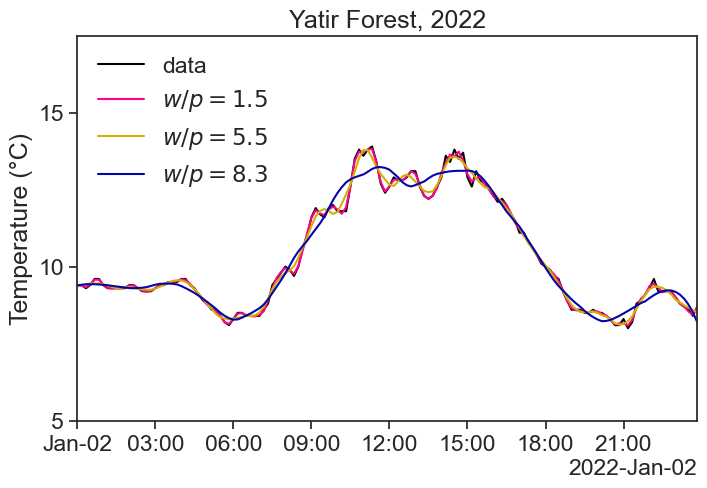
\includegraphics{seasonality/seasonal-decomposition_files/figure-pdf/cell-9-output-1.png}

}

\end{figure}

\hypertarget{hilbert-transform}{%
\chapter{Hilbert transform}\label{hilbert-transform}}

\part{Rates of change}

\hypertarget{derivatives}{%
\chapter{Derivatives}\label{derivatives}}

\hypertarget{finite-differences}{%
\chapter{Finite differences}\label{finite-differences}}

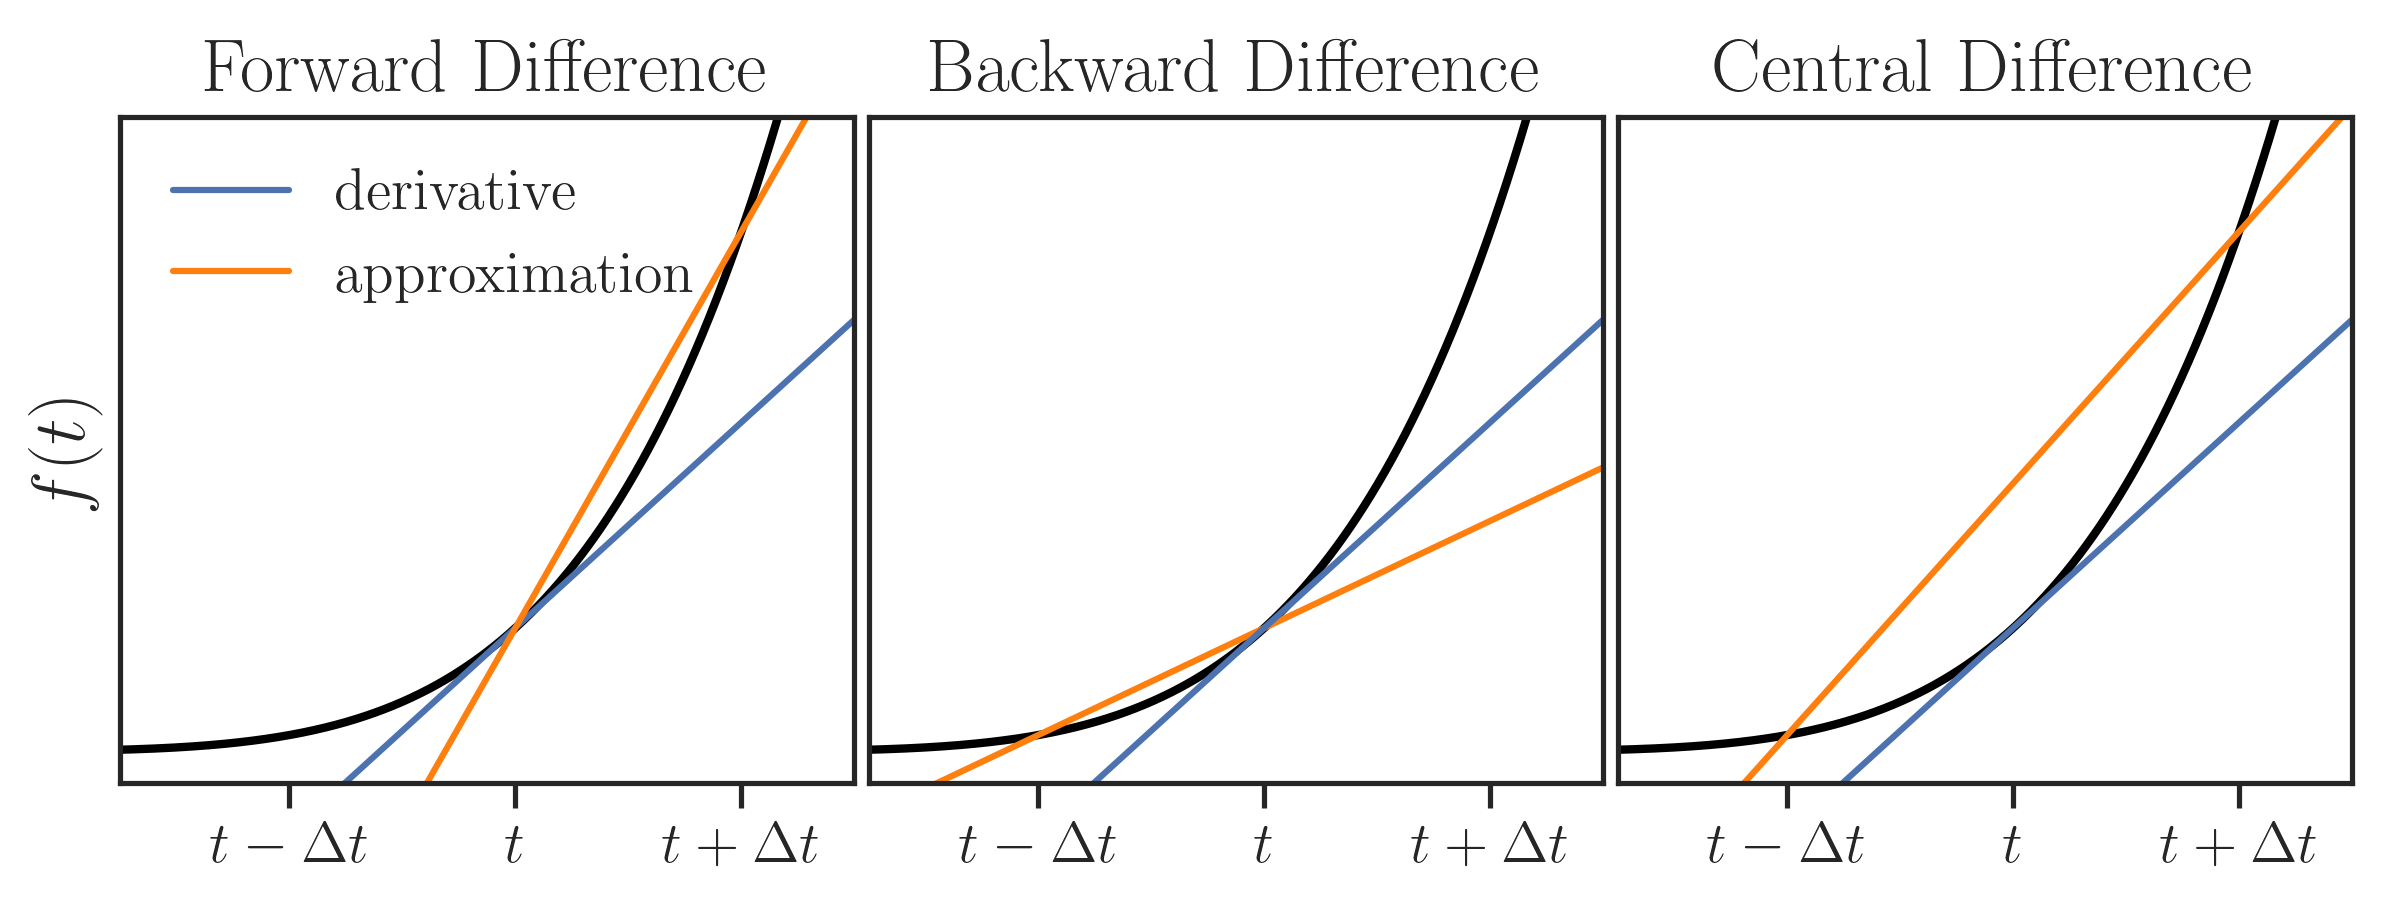
\includegraphics{rates-of-change/central_diff.png}

Definition of a derivative:

\[
\underbrace{\dot{f} = f'(t) = \frac{df(t)}{dt}}_{\text{same thing}} = \lim_{\Delta t \rightarrow 0} \frac{f(t+\Delta t) - f(t)}{\Delta t}.
\]

Numerically, we can approximate the derivative \(f'(t)\) of a time
series \(f(t)\) as

\begin{equation}\protect\hypertarget{eq-tpfdf}{}{
\frac{df(t)}{dt} = \frac{f(t+\Delta t) - f(t)}{\Delta t} + \mathcal{O}(\Delta t).
}\label{eq-tpfdf}\end{equation}

\marginnote{\begin{footnotesize}

The expression \(\mathcal{O}(\Delta t)\) means that the error associated
with the approximation is proportional to \(\Delta t\). This is called
\href{https://en.wikipedia.org/wiki/Big_O_notation}{``Big O notation''}.

\end{footnotesize}}

The expression above is called the \emph{two-point forward difference
formula}. Likewise, we can define the \emph{two-point backward
difference formula}:

\begin{equation}\protect\hypertarget{eq-tpbdf}{}{
\frac{df(t)}{dt} = \frac{f(t) - f(t-\Delta t)}{\Delta t} + \mathcal{O}(\Delta t).
}\label{eq-tpbdf}\end{equation}

If we sum together Equation~\ref{eq-tpfdf} and Equation~\ref{eq-tpbdf}
we get:

\begin{equation}\protect\hypertarget{eq-sum}{}{
\begin{aligned}
2\frac{df(t)}{dt} &= \frac{f(t+\Delta t) - \cancel{f(t)}}{\Delta t} + \frac{\cancel{f(t)} - f(t-\Delta t)}{\Delta t} \\
 &= \frac{f(t+\Delta t) - f(t-\Delta t)}{\Delta t}.
\end{aligned}
}\label{eq-sum}\end{equation}

Dividing both sides by 2 gives the \emph{two-point central difference
formula}:

\begin{equation}\protect\hypertarget{eq-twcdf}{}{
\frac{df(t)}{dt} = \frac{f(t+\Delta t) - f(t-\Delta t)}{2\Delta t} + \mathcal{O}(\Delta t^2). 
}\label{eq-twcdf}\end{equation}

Two things are worth mentioning about the approximation above:

\begin{enumerate}
\def\labelenumi{\arabic{enumi}.}
\tightlist
\item
  it is balanced, that is, there is no preference of the future over the
  past.
\item
  its error is proportional to \(\Delta t^2\), it is a lot more precise
  than the unbalanced approximations :)
\end{enumerate}

\marginnote{\begin{footnotesize}

To understand why the error is proportional to \(\Delta t^2\), one can
subtract the Taylor expansion of \(f(t-\Delta t)\) from the Taylor
expansion of \(f(t+\Delta t)\).
\href{https://home.cc.umanitoba.ca/~farhadi/Math2120/Numerical\%20Differentiation.pdf}{See
this, pages 3 and 4.}

\end{footnotesize}}

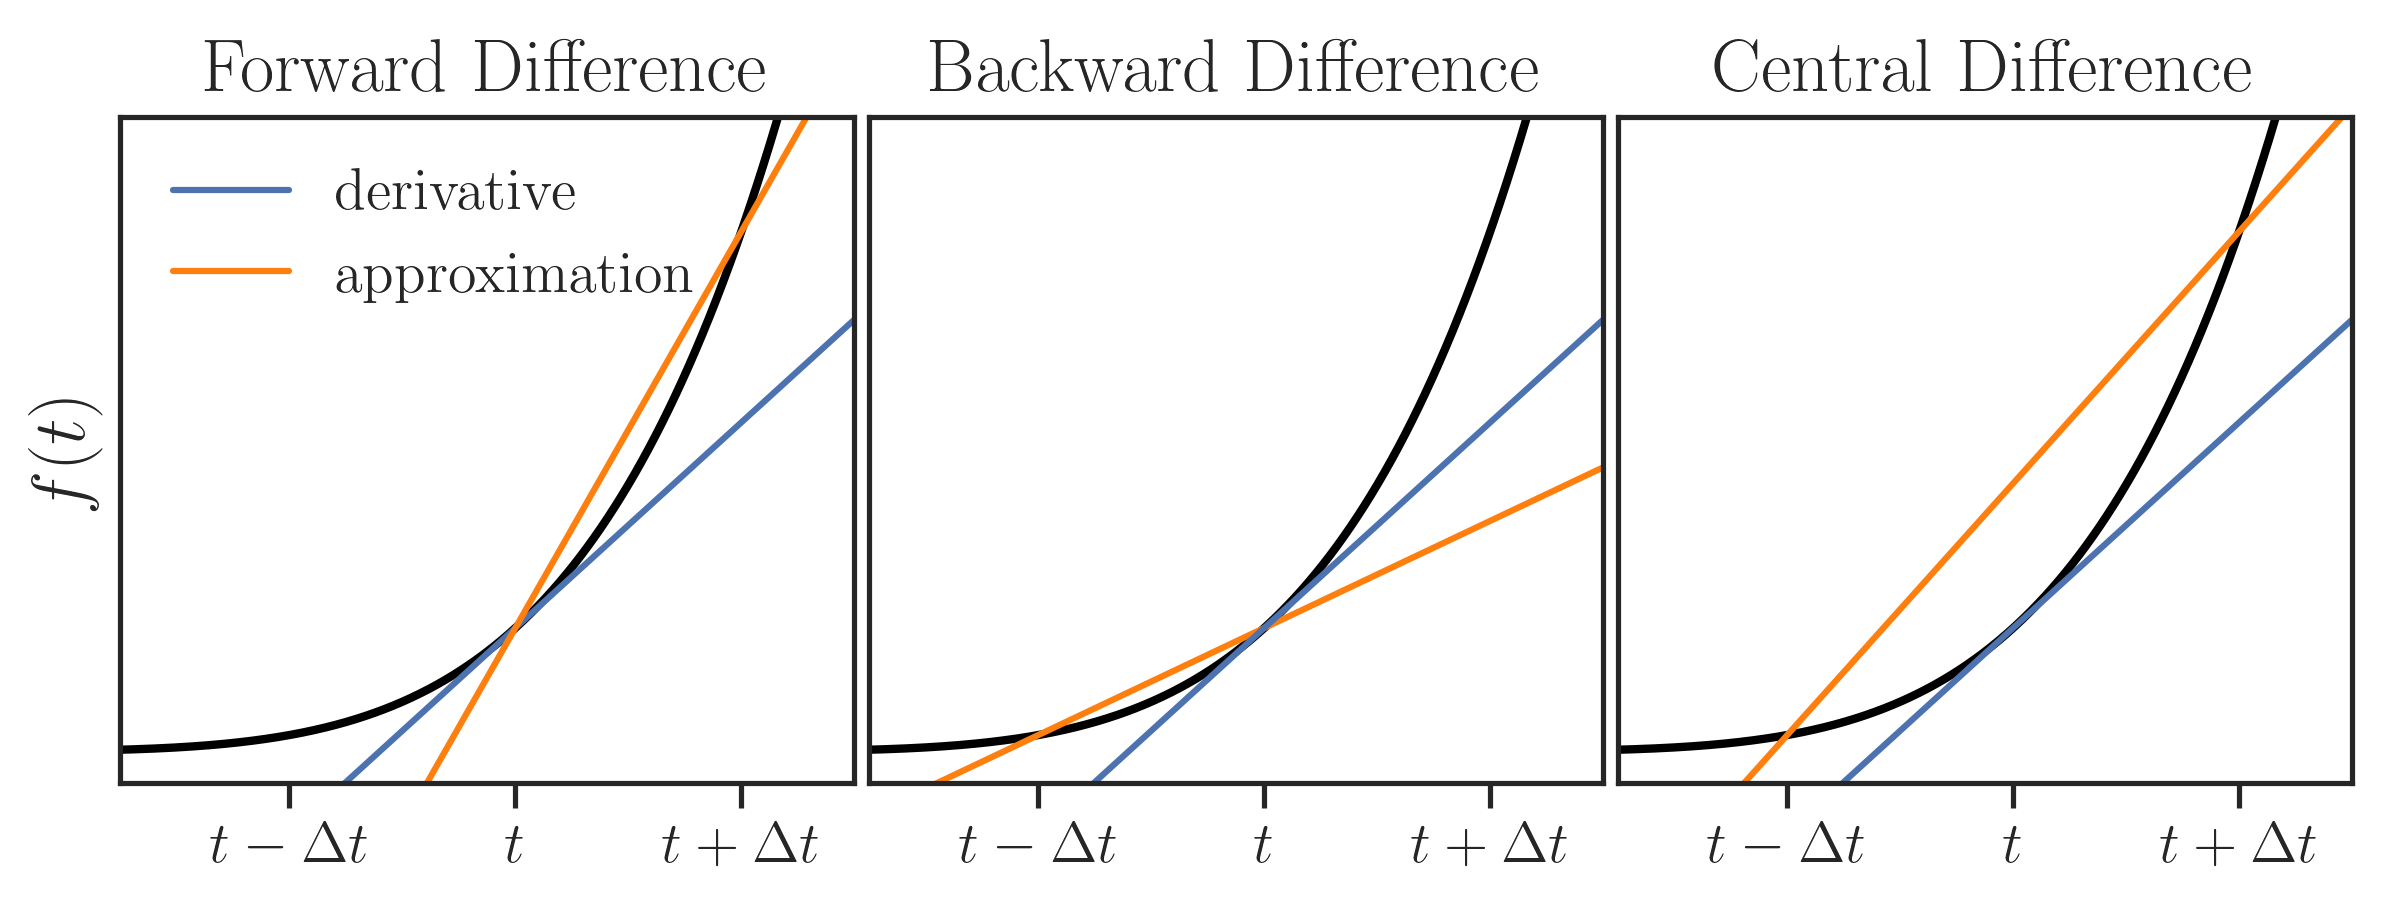
\includegraphics{rates-of-change/central_diff.png}

The function
\href{https://numpy.org/doc/stable/reference/generated/numpy.gradient.html}{\texttt{np.gradient}}
calculates the derivative using the central difference for points in the
interior of the array, and uses the forward (backward) difference for
the derivative at the beginning (end) of the array.

\marginnote{\begin{footnotesize}

The ``gradient'' usually refers to a first derivative with respect to
space, and it is denoted as \(\nabla f(x)=\frac{df(x)}{dx}\). However,
it doesn't really matter if we call the independent variable \(x\) or
\(t\), the derivative operator is exactly the same.

\end{footnotesize}}

Check out this
\href{https://gist.github.com/astrojuanlu/e4d47fec5d94d2224762a61680419eb2}{nice
example}.

\hypertarget{fourier-based-derivatives}{%
\chapter{Fourier-based derivatives}\label{fourier-based-derivatives}}

https://nirpyresearch.com/fourier-spectral-smoothing-method/

\hypertarget{loess-based-derivatives}{%
\chapter{LOESS-based derivatives}\label{loess-based-derivatives}}

\part{Forecasting}

\hypertarget{arima}{%
\chapter{ARIMA}\label{arima}}

\bookmarksetup{startatroot}

\hypertarget{technical-stuff}{%
\chapter*{Technical Stuff}\label{technical-stuff}}
\addcontentsline{toc}{chapter}{Technical Stuff}

\markboth{Technical Stuff}{Technical Stuff}

\hypertarget{operating-systems}{%
\section*{Operating systems}\label{operating-systems}}
\addcontentsline{toc}{section}{Operating systems}

\markright{Operating systems}

I recommend working with UNIX-based operating systems (MacOS or Linux).
Everything is easier.

If you use Windows, consider
\href{https://learn.microsoft.com/en-us/windows/wsl/install}{installing
Linux on Windows with WSL}.

\hypertarget{software}{%
\section*{Software}\label{software}}
\addcontentsline{toc}{section}{Software}

\markright{Software}

\href{https://www.anaconda.com/download}{Anaconda's Python distribution}

\href{https://code.visualstudio.com/download}{VSCode}

\hypertarget{python-packages}{%
\section*{Python packages}\label{python-packages}}
\addcontentsline{toc}{section}{Python packages}

\markright{Python packages}

\href{https://engineering.fb.com/2021/06/21/open-source/kats/}{Kats ---
a one-stop shop for time series analysis}\\
Developed by Meta

\href{https://www.statsmodels.org/stable/}{statsmodels} statsmodels is a
Python package that provides a complement to scipy for statistical
computations including descriptive statistics and estimation and
inference for statistical models.

\href{https://ydata-profiling.ydata.ai/docs/master/pages/use_cases/time_series_datasets.html}{ydata-profiling}\\
Quick Exploratory Data Analysis on time-series data.
\href{https://towardsdatascience.com/how-to-do-an-eda-for-time-series-cbb92b3b1913}{Read
also this}.

\bookmarksetup{startatroot}

\hypertarget{sources}{%
\chapter*{Sources}\label{sources}}
\addcontentsline{toc}{chapter}{Sources}

\markboth{Sources}{Sources}

\hypertarget{books}{%
\section*{Books}\label{books}}
\addcontentsline{toc}{section}{Books}

\markright{Books}

\href{https://www.data-to-viz.com}{from Data to Viz}

\href{https://clauswilke.com/dataviz/}{Fundamentals of Data
Visualization, by Claus O. Wilke}

\href{https://soilwater.github.io/pynotes-agriscience/intro.html}{PyNotes
in Agriscience}

\href{https://otexts.com/fpp3/}{Forecasting: Principles and Practice
(3rd ed), by Rob J Hyndman and George Athanasopoulos}

\href{https://github.com/erykml/Python-for-Finance-Cookbook-2E}{Python
for Finance Cookbook 2nd Edition - Code Repository}

\href{https://huji.primo.exlibrisgroup.com/permalink/972HUJI_INST/10ptda2/alma9920842016603701}{Practical
time series analysis,: prediction with statistics and machine learning,
by Aileen Nielsen}\\
The online edition of this book is available for Hebrew University staff
and students.

\href{https://huji.primo.exlibrisgroup.com/permalink/972HUJI_INST/10ptda2/alma9921049267803701}{Time
series analysis with Python cookbook : practical recipes for exploratory
data analysis, data preparation, forecasting, and model evaluation, by
Tarek A. Atwan}\\
The online edition of this book is available for Hebrew University staff
and students.

\href{https://huji.primo.exlibrisgroup.com/permalink/972HUJI_INST/10ptda2/alma9920845706703701}{Hands-on
Time Series Analysis with Python: From Basics to Bleeding Edge
Techniques, by B V Vishwas, Ashish Patel}\\
The online edition of this book is available for Hebrew University staff
and students.

\hypertarget{videos}{%
\section*{Videos}\label{videos}}
\addcontentsline{toc}{section}{Videos}

\markright{Videos}

\href{https://learning.oreilly.com/videos/times-series-analysis/9780136944515/}{Times
Series Analysis for Everyone, by Bruno Goncalves}\\
This series is available for Hebrew University staff and students.

\href{https://learning.oreilly.com/videos/time-series-analysis/00000G9DZPO7DJKE/}{Time
Series Analysis with Pandas, by Joshua Malina} This video is available
for Hebrew University staff and students.

\hypertarget{references}{%
\section*{References}\label{references}}
\addcontentsline{toc}{section}{References}

\markright{References}

\hypertarget{refs}{}
\begin{CSLReferences}{1}{0}
\leavevmode\vadjust pre{\hypertarget{ref-atwan2022time}{}}%
Atwan, Tarek A. 2022. \emph{Time Series Analysis with Python Cookbook:
Practical Recipes for Exploratory Data Analysis, Data Preparation,
Forecasting, and Model Evaluation}. Packt.

\leavevmode\vadjust pre{\hypertarget{ref-eilers2003perfect}{}}%
Eilers, Paul HC. 2003. {``A Perfect Smoother.''} \emph{Analytical
Chemistry} 75 (14): 3631--36. \url{https://doi.org/10.1021/ac034173t}.

\end{CSLReferences}



\end{document}
